\documentclass[final,3p,times,twocolumn]{elsarticle}
%\usepackage{natbib}
\usepackage{amsmath}
\usepackage{amstext}
\usepackage{amssymb}
\usepackage{array}
\usepackage{hyperref}
\usepackage{datetime}
\usepackage{url}
\usepackage{bm}
\usepackage{bbold}
%\usepackage{color}
\usepackage{graphicx}
\usepackage[dvipsnames]{xcolor}
\usepackage{epstopdf}
\usepackage{tikz}
\usepackage{float}
\usepackage{caption}
\usepackage{graphicx}
\usepackage{latexsym}
 \usepackage[a-1b]{pdfx}
\newcommand{\mat}[1]{\mathbf{#1}}                        % matrix
\newcommand{\sqmat}[1]{\mat{#1}^{\frac{1}{2}}}
\newcommand{\sqmatT}[1]{\mat{#1}^{\frac{\top}{2}}}
\newcommand{\tildemat}[1]{\tilde{\mat{#1}}}
\newcommand{\com}[1]{{\color{blue}@@@#1@@@}}             % comment for discussions
\newcommand{\bl}[1]{{\color{blue}#1}}                    % marks text changed in this revision
\newcommand{\blt}[1]{\texorpdfstring{\bl{#1}}{#1}}          % blue (sub)section title, safe in bookmarks


\begin{document}
\title{Bayesian Adaptive Portfolio Optimisation Exploiting Fully Probabilistic Design}

\author[1]{Tom\'{a}\v{s} Proch\'{a}zka and Miroslav K\'{a}rn\'{y}}%[<options>]
\ead{\{prochazka,school\}@utia.cas.cz}
\ead[url]{http://www.utia.cas.cz/AS}
\affiliation[1]{organization={The Czech Academy of Sciences, Institute of Information Theory and Automation, Department of Adaptive Systems},
            addressline={Pod Vod\'{a}renskou v\v{e}\v{z}\'{i} 1143/4},
            city={Prague 8},
            postcode={182 00},
           country={Czech Republic}}

\begin{abstract} Web of Science reports more than eighteen thousand items concerning portfolio optimisation, and Google Scholar reports more than three and a half million. It indicates the topic's importance and provokes the question of
whether it makes sense to add a new item to this pile.
The paper positively answers it by offering:\\
$\checkmark$  Bayesian learning of an autoregressive model with exogenous variables
that: $\bullet$ optimally chooses the conjugate prior probability density function of unknown parameters; $\bullet$ \bl{estimates the model structure by a genetic search over an exact Bayesian criterion}; $\bullet$ tracks the parameter changes via an optimised data-based forgetting, which robustifies \bl{estimation against outlying observations}; $\bullet$  employs a safe updating of a sufficient statistic;\\
$\checkmark$  Use of the autoregressive model for expected multi-step quadratic-loss design of the decision policy that:
$\bullet$ relies on numerically safe, feasible square root optimisation with receding-horizon design; $\bullet$ elicits optimal weights in quadratic loss, exploiting the fully probabilistic design of the decision policy that guarantees proper handling of risks in a non-traditional but consistent way; $\bullet$ opens a way to off-line design with Thompson's sampling of parameters, which leads to a reliable prediction of the quality of the obtained policy.

\bl{The solution is complete in the sense that every step, from the choice of the prior to the constrained design, is derived within a single framework.} Our solution can also be applied to many other decision-making problems. \bl{Practically, the number of hyperparameters is small, and the experiments identify the two that matter. A paired comparison on 200 random portfolios and four market windows against standard benchmarks (equal-weight, minimum-variance, mean-variance, the S\&P~500), an ablation of every component, a sensitivity study, and stress tests on synthetic data with known parameters are reported with the released code. The policy has consistently smaller drawdowns than mean-variance allocation and its adaptive forgetting rejects outlying observations as designed; it does not outperform the equal-weight portfolio after transaction costs, and the experiments locate the reason in the elicitation of the risk weight and in the strength of the optimal prior.}
\end{abstract}

\maketitle
\journal{Omega}

\noindent\textbf{Keywords:} portfolio optimisation, probabilistic modelling, adaptive decision-making, fully probabilistic design\footnote{This work was supported by CTU SGS25/167/OHK4/3T/14, EU-COST Action CA24136\,\&\,by the TALISMAN Laboratory.}

\subsection*{Highlights}
\begin{itemize}
\item complete, consistent, and analytical solution of the hard trading problem
\item structure estimation and hierarchical priors
\item \bl{novel adaptive forgetting, rejecting outlying observations}
\item novel elicitation of the risk-aware quadratic loss
\item \bl{numerically safe implementation and few tuning knobs}
\item \bl{paired benchmark, ablation and stress-test study with released code}
 \end{itemize}

%\tableofcontents
%%%%%%%%%%%%%%%%%%%%%%%%%%%%%%%%%%%%%%%%%%%%%%%%%%%%%%%%%%%%%%
\section{Introduction} \label{s:introduction}
The paper presents a structured, methodologically consistent approach to portfolio optimisation. It complements, improves and combines all the steps needed for an adaptive, feasible, and complete solution. It utilizes many known practices and results from Bayesian statistics, \cite{Pet:81,KarKul:88,Kar:25a}, tracking of parameter changes, \cite{Kul:93a}, linear-quadratic adaptive regulation (LQR), \cite{AstWit:94}, especially in the fully probabilistic design (FPD) version, \cite{Kar:19}, quadratic optimisation \cite{dostal2009optimal},  and an established search heuristics, \cite{haldurai2016study}. The main contribution of this article is unifying, improving upon, and connecting these parts. 

The paper provides a systematic approach to decision-making that leverages the strong theoretical foundation and minimal requirements on user inputs. The presented design is useful not only on financial markets but, with slight modifications, to a wide variety of dynamic decision-making problems.

\subsection*{On Related Work}

The research in the field of quantitative portfolio optimisation spans a vast area of different views on the problem and its solution. To illustrate this, it suffices to take recent samples from this journal \cite{BenLeaPue:25,LiGaoShu:26,LyuWuGuoGuChi:24}.

%\cite{AliWanWan:25,Laietal:20,ZhaWan:26}.

Classical approaches \cite{michaud1989markowitz} frame the portfolio choice as a dual optimisation, where expected returns are maximised,  and variance is minimised. Many innovative approaches exist. For instance \cite{abbracciavento2025model}, which optimises the objective function tuned to directly meet users' (investors') preferences like an adverse to risk, a diversification priority and other user-specific needs. However, the complex choice among many possible configurations is left to the user's responsibility. This hinders the approach strength. It also makes an objective evaluation of the gain in performance hard.

The systematic way to the specific version of the common preference elicitation problems \cite{ChePu:04} is a significant part of our solution. It optimises expected quadratic loss expressing portfolio-choice objectives. Together with the adopted, online estimated, autoregressive returns model with exogenous variables  (ARX), \cite{Pet:81}, the solution becomes a version of the linear quadratic regulator task, which is so common in the control domain, \cite{LQRPSOOptKalmanfilter}. The use of novel adaptive forgetting \cite{Kar:25} makes the resulting allocation more robust against black swan events, notoriously connected with financial markets \cite{bogle2008black}.

In the portfolio optimisation context, the LQR setting was applied  in \cite{cura2009particle} to optimise the efficient frontier, meaning the relationship between portfolio returns and their variance. There, LQR is enhanced by particle swarm optimisation. LQR setup also applies to related tasks. For example, high-frequency trading is addressed as the continuous-time LQR for hedging portfolios on the options market. Unlike the multitude of academic papers, this solution considers transaction costs \cite{hedgingundertransactioncosts}.

 Other typical instances of portfolio optimisation, including machine learning, are reviewed by \cite{gunjan2023brief}. The range of applied methods and the variability in the results indicate that the portfolio optimisation problem is far from being solved.

\subsection*{Paper's Aim}
This work aims to develop a solution that: $\bullet$ does not leave out any of its important subtasks;  $\bullet$ is as deductive as possible; $\bullet$ relies as little as possible on the user's tuning of the hyperparameters.

\subsection*{Notation}  We consider a finite number of assets $N\in \mathbb{N} =$ natural numbers. The returns of individual assets are observed in discrete time $t\in \mathbb{N} \cup \{0\}$. They are denoted as  $y_{t}\in [-1,+\infty)^N$ with $y_{t}$ being an $N$-vector containing the returns of all $N$ assets indexed by $i\in\{1,\dots N\}$  $(y_{i,t})_{i=1}^N$. All of the considered assets are denominated in United States Dollar (USD). We do not consider currency risks\footnote{Assets denominated in currencies other than the USD carry the risk that this currency will be devalued in comparison to the USD, which is still universally accepted as a safe-haven asset.}.

We use $z_{t}\in \mathbb{R}^{\rho},\ \rho \geq N$, $\mathbb{R}$ denotes the real line, a $\rho$-vector of other observed variables, possibly exogenous factors, at time $t$, as the regressors. $d_{i,t}\in[0,1)$, $i\in\{1,\ldots,N\}$, is the transaction cost associated with the asset $i$ at time $t$.

The opted allocation of funds forms an $N$-vector $a_{t}$, which expresses percentages of the portfolio the respective assets occupy. This is the action at time $t$ in our decision-making task. We consider a spot portfolio with no leverage and short-selling. This poses constraints on the action space $ \{a\in\mathbb{R}^N\mid \mat{1}^{\top}a= 1, a\geq 0\}$.

The collection of all data up to the time step $t$ is $\mathcal{D}^{(t)} = \big(\mathcal{D}^{(t-1)},(y_{t}, z_{t}, d_{t})\big)$, $\mathcal{D}^{(0)}$ marks prior knowledge.

\subsection*{Explanation Basis and Layout}
The market returns are modelled by a multivariate ARX model, Sec.\ \ref{s:model}. Its parameters are unknown, and the needed predictor is gained via Bayesian methodology, \cite{Pet:81}. We cover the choice of the prior probability density function (PDF), Sec.\ \ref{s:prior}, the model-structure estimation, Sec.\ \ref{s:SE}, and the parameter tracking with forgetting Sec.\ \ref{s:forgetting}.

Parameter estimates are updated in real time. The newest point parameter estimate inserted into the ARX model provides the predictor that suits the policy optimisation formulated as an LQR task in Sec.\ \ref{s:lqrsection}.

The policy design starts with the specification of the loss function that quantitatively expresses the user's desire to maximise expected returns, while including transaction costs and respecting uncertainty about future returns. The quantitative specification exploits the fully probabilistic design of decision policies, \cite{karny2022fully}.

FPD extends classical decision-making theory,
\cite{Deg:70,FeiShw:02}, and stochastic control, \cite{Ber:17}, see Sec.\ \ref{s:FPD}. It fits the adopted Bayesian estimation, \cite{Pet:81}, \cite{Bretthorst1990}, and helps us to integrate uncertainty-induced risks.

The policy optimisation for the given quadratic loss and the ARX model is in Sec.\ \ref{s:lqrsection}. Similarly to the parameter estimation in Sec.\ \ref{s:model}, it cares about an efficient, numerically safe, square root implementation.

%The Bayesian setup and the FPD framework allow us to employ Thompson's parameter sampling, \cite{Rusetal:18}. It serves as a tool for a prediction of the success of the designed policy without practically closing the decision loop, Sec.\ \ref{s:exploration}.

Sec.\ \ref{s:experiments} \bl{reports a paired comparison with standard portfolio benchmarks, an ablation of every component of the pipeline, a sensitivity study and stress tests; it identifies the parts that carry the performance and the two design elements that limit it.} The paper is closed by comments in Sec.\ \ref{s:conclusions}. 
\subsection*{Pipeline} \label{s:pipeline}
The proposed portfolio optimisation uses (mostly well-known) techniques from Bayesian statistics and optimisation. The pipeline of our process is shown in Fig.\ \ref{fig:pipelinetikz}.
\usetikzlibrary{shapes, arrows.meta, positioning, fit, calc}

\definecolor{myblue}{HTML}{B4C8DC}   % Light blue (fill)
\definecolor{darkerblue}{HTML}{8C9FB5} % Border
\definecolor{textblue}{HTML}{0A2846}   % Optional dark blue text
\begin{figure}[!ht]
    \centering
\begin{tikzpicture}[
    block/.style={rectangle, draw=textblue, fill=myblue, rounded corners,
                  text width=2.5cm, minimum height=1.0cm, align=center, font=\sffamily\small},
    decision/.style={diamond, draw=textblue, fill=darkerblue,
                     text width=2.5cm, minimum height=1cm, align=center, font=\sffamily\small},
    line/.style={draw, -{Latex[length=3mm, width=2mm]}, thick, textblue},
    textlabel/.style={pos=0.5, font=\sffamily\tiny, textblue},
    every node/.style={text=textblue}
]

    % Nodes
    \node (market) [block] {market};
    \node (rest_of_world) [block, right=1cm of market] {rest of the world};
    \node (model) [block, below=1cm of market] {adaptive model learning};
    \node (opt_prior) [block, right=1cm of model] {prior PDF choice \& structure estimation};
    \node (LQR) [block, below=1cm of model] {preference quantification \& optimization};
    \node (opt_alg) [block, below=1cm of LQR] {allocation};
    \node (user) [block, below=of opt_prior, right=of opt_alg] {user};

    % Connections
    \draw [line] (market.south) -- node[textlabel, right, font=\large] {$y_t$} (model.north);
    \draw [line] (opt_prior.west) -- (model.east);
    \draw [line] (rest_of_world) to node[textlabel, above, pos=0.5, font=\large] {$z_t$} (model);
    \draw [line] (model.south) -- node[textlabel, right, font=\normalsize] {predictor} (LQR.north);
    \draw [line] (LQR.south) -- node[textlabel, right, font=\normalsize] {policy} (opt_alg.north) ;

    % dashed line of returns to user
    \draw [dashed] (opt_alg.east) -- node[textlabel, above, pos=0.5, font=\large] {
$a_{t}^{\top}y_{t}$} (user.west);

    % Two-way arrow for Market and Rest of the World
    \draw [line, -] (market.east) -- (rest_of_world.west);

    % User loops
    \draw [line] (user.north) -- (opt_prior.south) node[textlabel, right, pos=0.65, font=\normalsize] {hyperparameter};
    \draw [line] (user.north) |- (LQR.east) node[textlabel, left, pos=0.1, above, pos=0.75, font=\normalsize] {constraints};

    % Feedback from LQR
    \draw [line] (rest_of_world.south) --(opt_prior.north);

\end{tikzpicture}
   \caption{\emph{Solution pipeline}:
   The market produces the observed $y_{t}$, which are returns of assets in the user's portfolio at time $t$. The rest of the world, which preserves past market data, gives information $z_{t}=(a_{t},x_{t-1})$ potentially useful for predicting the said returns. Data serves to model structure estimation, choice of Bayesian prior and forgetting. The learned model $(\mbox{available knowledge})\rightarrow y_{t}$ also serves for a quantitative expression of the user's wishes and for the optimal allocation $a_{t}$ of the funds before $y_{t}$ realisation. After it, the user receives the return $a_{t}^{\top}y_{t}$.
   }
    \label{fig:pipelinetikz}
\end{figure} 
\section{Complete Learning of the Returns Model} \label{s:model}
A multivariate autoregressive model with exogenous variables serves well for predicting market returns $y_{t}$.  This is a simple yet powerful common model.  It allows for an efficient Bayesian parameter estimation and gives the returns' predictor. The ARX model reads
\begin{equation}\label{e:linearmodel}
    y_{t} = \mat{P}^{\top}z_{t} + e_{t},\ z^{\top}_{t}=[a^{\top}_{t},x^{\top}_{t-1}] \quad e_{t} \sim \mathcal{N}(0, \mat{\Sigma}),
\end{equation}
where $\mat{P}$ is $(\rho, N)$-matrix of regression coefficients, $x_{t-1}$ is a vector of regressors. The $N$-vector $e_{t}$ is normally distributed noise with zero mean and covariance $\mat{\Sigma}$. The noise $e_{t}$ is independent of $z_{t}$ and $e_{\tau}$ for $\tau<t$.

$\mat{P}$ and $\mat{\Sigma}^{-1}$ form an unknown parameter $\theta = (\mat{P}, \mat{\Sigma}^{-1})\in \Theta$ of the model. The corresponding parametric model, PDF marked throughout $p(\cdot)$ for the join, prior, posterior and predictive PDFs, $m(\cdot)$ for the returns model, and $r(\cdot)$ for rules of the decision policy, reads $  m(y_{t}|a_{t}, \mathcal{D}^{(t-1)}, \theta)$

\begin{equation}
    \label{e:cPDFlinearmodel}
\hspace*{-4ex}   = \frac{\exp \left[-\frac{1}{2}(y_{t} -\mat{P}^{\top}z_{t})^{\top}\mat{\Sigma}^{-1}(y_{t} -\mat{P}^{\top}z_{t})\right]}{(2\pi)^{\frac{N}{2}}|\mat{\Sigma}|^{\frac{1}{2}}}.
\end{equation}
To get the predictor $p(y_{t+1}|a_{t+1}, \mathcal{D}^{(t)})$,
where $\mathcal{D}^{(t)}$ marks knowledge available at time $t$, we use Bayes' rule
\begin{equation}
\label{e:parametersPDF}
p(\theta|\mathcal{D}^{(t)}) = \frac{p(\mathcal{D}^{(t)}|\theta,\mathcal{D}^{(0)})p(\theta|\mathcal{D}^{(0)})}
{\int_{\Theta}p(\mathcal{D}^{(t)}|\theta,\mathcal{D}^{(0)})p(\theta|\mathcal{D}^{(0)})d\theta}.
\end{equation}
As usual, the prior knowledge $\mathcal{D}^{(0)}$ in the prior PDF $p(\theta)=p(\theta|\mathcal{D}^{0})$ and other PDFs are implicitly present.

The chain rule for PDFs provides the joint PDF of all available data conditioned on the unknown $\theta$
(and $\mathcal{D}^{(0)}$)
\begin{equation}
 \label{e:chainrule}
    \hspace*{-4ex}
p(\mathcal{D}^{(t)}|\theta) = \prod_{\tau = 1}^{t} m(y_{\tau}|a_{\tau}, \mathcal{D}^{(\tau-1)}, \theta)r(a_{\tau}|\mathcal{D}^{(\tau-1)}, \theta)
\end{equation}
The parameter $\theta\in \Theta$ is unknown to the user who chooses the actions. Thus, PDFs describing the user's policy formed by randomised rules $r$ meet the natural conditions of control, \cite{Pet:81}, $\big(r(a_{t}|\mathcal{D}^{(t-1)}, \theta) = r(a_{t}|\mathcal{D}^{(t-1)})\big)_{t=1}^{H}$, where the considered horizon $H\in \mathbb{N}$. Under them, (\ref{e:parametersPDF}) is
\begin{eqnarray}
\nonumber
\hspace*{-4ex}p(\theta|\mathcal{D}^{(t)}) &=& \frac{l(\mathcal{D}^{(t)},\theta)p(\theta)}{J(\mathcal{D}^{(t)})},
\mbox{ where the denominator is}\\
\nonumber
\hspace*{-4ex}J(\mathcal{D}^{(t)})&=&
\int_{\Theta} l(\mathcal{D}^{(t)},\theta)p(\theta)d\theta,\ \mbox{ and}\\
\label{e:likelihooddef}
\hspace*{-4ex}l(\mathcal{D}^{(t)},\theta) &=&\prod_{\tau = 1}^{t} m(y_{\tau}|a_{\tau}, \mathcal{D}^{(\tau-1)}, \theta)
\end{eqnarray}
is the likelihood function, i.e., the factor of the PDF (\ref{e:chainrule}) modelling environment (at fixed $\mathcal{D}^{(t)}$) depending on the possible parameter values.

Using the likelihood function and the denominator (\ref{e:likelihooddef}) plus marginalisation, \cite{Pet:81}, we obtain the exact predictor of future returns
\begin{equation}
    \label{e:returnsPDF}
    p(y_{t+1}| a_{t+1}, \mathcal{D}^{(t)}) = \frac{J(\mathcal{D}^{(t+1)})}{J(\mathcal{D}^{(t)})}.
\end{equation}
The likelihood (\ref{e:likelihooddef}) for the PDF (\ref{e:cPDFlinearmodel}) can be expressed as
\begin{eqnarray*}
    %\label{e:likelihoodwithV}
    &&l(\mathcal{D}^{(t)}, \theta) = (2\pi)^{-N\frac{t}{2}} |\mat{\Sigma}|^{-\frac{t}{2}}\\
 \nonumber
  &\times&
   \exp\bigg\{-0.5\text{tr}\Big[\mat{\Sigma}^{-1}
   \begin{pmatrix}
    -\mat{I}&
    \mat{P}^{\top}
    \end{pmatrix}
    \tildemat{V}_{t}
    \begin{pmatrix}
    -\mat{I}\\
    \mat{P}
    \end{pmatrix}\Big]\bigg\}.
\end{eqnarray*}
The extended information matrix $\tildemat{V}_{t}$ and the counter $t$ form the sufficient statistic, i.e., $p(\theta|\mathcal{D}^{(t)})\propto p(\theta|\tildemat{V}_{t},t,\mathcal{D}^{(0)})$. They encapsulate the collected data and enrich the prior knowledge $\mathcal{D}^{(0)}=(\mat{V}_{0},\Delta_{0})$ to, see (\ref{e:linearmodel}),
\begin{eqnarray}
 \label{e:Vmatrix}
    \mat{V}_{t} &=& \sum_{\tau = 0}^{t}
    \begin{pmatrix}
        y_{\tau}\\ z_{\tau}
    \end{pmatrix}
    \begin{pmatrix}
        y_{\tau}^{\top} z_{\tau}^{\top}
    \end{pmatrix} + \mat{V}_{0} = \tildemat{V}_{t} + \mat{V}_{0}\\
  \nonumber      
     \Delta_{t}&=& t + \Delta_{0}.
\end{eqnarray}

The matrix $\mat{V}_{0} >0$ and degrees of freedom $\Delta_{0}>\rho$ reflect the prior beliefs about $\theta$ quantified by conjugate (self-reproducing) Gauss-inverse-Wishart PDF, \cite{Pet:81,Zel:76}. The optimised choice of $\mat{V}_{0}$,  $\Delta_{0}$ is in Sec.\ \ref{s:prior}.
 The matrix (\ref{e:Vmatrix}) is partitioned as
\begin{equation}
\label{e:Vpartition}
    \mat{V}_{t} = \left(\begin{array}{cc}
        \mat{V}_{y,t} & \mat{V}_{zy,t}^{\top} \\
        \mat{V}_{zy,t} & \mat{V}_{z,t}
    \end{array}\right),\hspace*{2ex}\mat{V}_{y,t}\in \mathbb{R}^{N,N},
\end{equation}
and the prior $\mat{V}_{0}$ is partitioned in the same way. The posterior likelihood with this prior is rewritten into
\begin{eqnarray}
\label{e:likelihood}
&&\hspace*{-4ex}l(\mathcal{D}^{(t)},\theta)p(\theta)\\
\nonumber
&&\hspace*{-4ex}=\frac{\exp\left[-\frac{1}{2}\text{tr}\left(\mat{\Sigma}^{-1} (\mat{P} - \hat{\mat{P}}_{t})^{\top}\mat{V}_{z,t}(\mat{P} - \hat{\mat{P}}_{t}) + \mat{\Sigma}^{-1} \mat{\Lambda}_{t}\right)\right]}{(2\pi)^{N\frac{\Delta_{t}}{2}} |\mat{\Sigma}|^{\frac{\Delta_{t}}{2}}}.
\end{eqnarray}
The posterior parameter PDFs are
\begin{eqnarray}
\nonumber
&&\hspace*{-4ex} p(\mat{P}|\mathcal{D}^{(t)}, \mat{\Sigma}^{-1})= \\
\nonumber
&&\hspace*{-4ex}\frac{\exp\left[-\frac{1}{2}\text{tr}\left(\mat{\Sigma}^{-1}(\mat{P} - \hat{\mat{P}}_{t})^{\top}\mat{V}_{z,t}(\mat{P}-\hat{\mat{P}}_{t})\right)\right]}{(2\pi)^{\frac{\rho N}{2}}|\mat{V}_{z,t}|^{-\frac{N}{2}}|\mat{\Sigma}|^{\frac{\rho}{2}}}\\
\label{e:PDFSigma}
&&\hspace*{-4ex}p(\mat{\Sigma}^{-1}|\mathcal{D}^{(t)})=\\
\nonumber
&&\hspace*{-4ex}\frac{|\mat{\Lambda}_{t}|^{\frac{\Delta_{t}-\rho+N+1}{2}}|\mat{\Sigma}|^{-\frac{\Delta_{t}-\rho}{2}}
\exp\left[-\frac{1}{2}\text{tr}\left(\mat{\Sigma}^{-1}\mat{\Lambda}_{t}\right)\right]}
{(2^{\Delta_{t}-\rho+N+1}\pi^{\frac{N-1}{2}})^{\frac{N}{2}}\prod_{j=1}^N\Gamma\left(\frac{\Delta_{t}-\rho+N+2-j}{2}\right)}.
\end{eqnarray}
They exploit the analytical form of $J(\mathcal{D}^{(t)})$
(\ref{e:likelihooddef}), \cite{Pet:81},
\begin{eqnarray}
\nonumber
J(\mathcal{D}^{(t)})&=&J(\mat{V}_{t},\Delta_{t})=
(2\pi)^{\frac{\rho N}{2}}|\mat{V}_{z,t}|^{-\frac{N}{2}}
|\mat{\Lambda}_{t}|^{-\frac{\Delta_{t}-\rho+N+1}{2}}\\
\label{e:JARX}
&&\hspace*{-14ex}\times\,
(2^{\Delta_{t}-\rho+N+1}\pi^{\frac{N-1}{2}})^{\frac{N}{2}}
\prod_{j=1}^N\Gamma\left(\frac{\Delta_{t}-\rho+N+2-j}{2}\right)\\
\label{e:points}
&&\hspace*{-12ex}\hat{\mat{P}}_{t}=\mat{V}_{z,t}^{-1}\mat{V}_{zy,t},\ \mat{\Lambda}_{t}=\mat{V}_{y,t}
-  \mat{V}_{zy,t}^{\top}\mat{V}_{z,t}^{-1}\mat{V}_{zy,t}.
\end{eqnarray}
 The maxima of these PDFs are achieved at $\mat{P} = \hat{\mat{P}}_{t}$ and $\hat{\mat{\Sigma}}_{t}^{-1} = \Delta_{t}\mat{\Lambda}_{t}^{-1}$, respectively. The PDFs (\ref{e:PDFSigma}) and the denominator (\ref{e:JARX}) are exploited later on.

Often, regressors are (almost) collinear, \cite{Linetal:22}. Then, the sub-matrix $\mat{V}_{z,t}$ is poorly conditioned, which makes evaluations of the posterior PDF non-robust. This is resolved by updating the square root of the (positive semi-definite) matrix $\mat{V}_{t}$, \cite{GolLoa:12}. The version suited to all learning parts is
\begin{equation}
    \label{e:VdecompositiontoG}
    \mat{V}_{t} = \mat{G}_{t}\mat{G}_{t}^{\top}=\mat{G}_{t-1}\mat{G}_{t-1}^{\top}+
    \begin{pmatrix}
        y_{t}\\ z_{t}
    \end{pmatrix}
    \begin{pmatrix}
        y_{t}^{\top} z_{t}^{\top}
    \end{pmatrix},
\end{equation}
where $\mat{G}_{t}$ is an upper triangular matrix. The square root is partitioned as $\mat{V}_{t}$ in (\ref{e:Vpartition}), giving
\begin{equation*}
\mat{V}_{t}=\mat{G}_{t}\mat{G}_{t}^{\top} =
\left(\begin{array}{cc}
    \mat{G}_{y,t}\mat{G}_{y,t}^{\top} + \mat{G}_{zy,t}\mat{G}_{zy,t}^{\top}  & \mat{G}_{zy,t}\mat{G}_{z,t}^{\top} \\ \mat{G}_{z,t}\mat{G}_{zy,t}^{\top} &  \mat{G}_{z,t}\mat{G}_{z,t}^{\top}
     \end{array}\right).
\end{equation*}
It provides the maximum a posteriori likelihood point estimates (\ref{e:points}) of unknown $\mat{P}$, $\mat{\Sigma}^{-1}$. The maximum of (\ref{e:PDFSigma}) is reached by minimising over $\mat{P}$ the quadratic norm
\begin{equation*}
\left|\left|\left(\begin{array}{cc}
    \mat{G}_{y,t}^{\top} & \mat{O}\\ \mat{G}_{zy, t}^{\top} & \mat{G}_{z,t}^{\top}
\end{array}\right)
\begin{pmatrix}
    -\mat{I} \\ \mat{P}
\end{pmatrix}\right|\right|^2,
\end{equation*}
$\mat{O},\,\mat{I}$ are zero and unit matrix, respectively.
This, together with simple maximisation over $\Sigma$, gives
\begin{equation}
\label{e:leastsquaresPwithG}
 \hat{\mat{P}}_{t} = \mat{G}_{z,t}^{-\top}\mat{G}_{zy,t}^{\top},\hspace*{2ex}
   \hat{\mat{\Sigma}}_{t}=\Delta_{t}\mat{\Lambda}_{t} \mbox{ with }   \mat{\Lambda}_{t} = \mat{G}_{y,t}\mat{G}_{y,t}^{\top}.
\end{equation}
The update $\mat{G}_{t-1}\rightarrow^{(y_{t}^{\top}\ z_{t}^{\top})} \mat{G}_{t}$ equivalent to (\ref{e:VdecompositiontoG}) involves one, numerically stable, orthogonal rotation, \cite{Bir:77}. Moreover, it allows simple evaluations of determinants as products of diagonal entries of square root factors, $|\mat{V}_{z,t}|=\prod_{k=1}^{\rho}G_{kk,z,t}^{2}$ and $|\mat{\Lambda}_{t}|=\prod_{k=1}^{N}G^{2}_{kk,y,t}$. They are needed whenever the denominator $J(\cdot)$ (\ref{e:likelihooddef}) is used, see Secs.\ \ref{s:SE} and \ref{s:forgetting}. 
\subsection{Optimal Hierarchical Choice of Prior PDF}\label{s:prior}
For the inspected model (\ref{e:linearmodel}), the conjugate prior is the Gaussian-inverse-Wishart PDF. The prior PDF is specified by $(\mat{V}_{0}, \Delta_{0})$, where $\mat{V}_{0} > 0$ is a prior extended information matrix and  $\Delta_{0} > \rho$  is the prior degrees of freedom. Their influence
on the estimation process is significant, especially on the structure estimation performed in off-line mode on $\bar{t}$ data records, see Sec.\ \ref{s:SE}.

The paper \cite{Kar:25a} provides the optimal choice $({\mat{V}}_{0}, {\Delta}_{0})$ by maximising the marginal likelihood as a function of the explicitly expressed prior knowledge
\begin{equation*}
l(\mathcal{D}^{(\bar{t})}|\mat{V}_{0}, \Delta_{0}) := \int_{\Theta}p(\mathcal{D}^{(\bar{t})}|\theta)p(\theta|\mat{V}_{0},\Delta_{0})d\theta=
\frac{J(\mat{V}_{\bar{t}},\Delta_{\bar{t}})}{J(\mat{V}_{0},\Delta_{0})}
\end{equation*}
under the weakest common constraint that $(\mat{V}_{0}, \Delta_{0})$ must make the prior PDF proper. The mentioned paper proves the existence of this extreme, gives its form, and verifies its positive influence.

Operationally, the construction form $\bar{t}$ data records is as follows. First, we map the data on the square root $\tilde{\mat{G}}_{\bar{t}}$ of the extended information matrix with zero prior
\begin{equation*}
%\label{e:matrixVforpriorconstruction}
\tilde{\mat{V}}_{\bar{t}} = \sum_{\tau=1}^{\bar{t}} \begin{pmatrix}
    y_{\tau}\\ z_{\tau}
\end{pmatrix}\begin{pmatrix}
    y_{\tau}^{\top}  z_{\tau}^{\top}
\end{pmatrix} + \mat{O}=\tilde{\mat{G}}_{\bar{t}}\tilde{\mat{G}}_{\bar{t}}^{\top}.
\end{equation*}
It depends on the processed data $( y_{\tau}^{\top}  z_{\tau}^{\top})_{\tau=1}^{\bar{t}}$ only.

Then, we select a scalar tuning parameter $\mu \in (0, 1)$. This scalar optional parameter controls the shrinkage strength of the resulting prior PDF. The optimal prior degrees of freedom $\Delta_{0}$ are found by numerically solving the next nonlinear scalar equation with a unique solution
\begin{equation*}
%\label{e:solve_v0}
-\frac{1}{2} \ln(\mu) = \frac{\frac{1}{2}(1 - \mu)\bar{t}}{ \bar{t} + (1 - \mu)\Delta_{0}} + h(\Delta_{0}) - h(\bar{t} + \Delta_{0}),
\end{equation*}
where $\bar{t}$ is the number of processed data, and $h(\Delta)$ is a function involving the digamma function $\Psi(\chi) = \frac{\mathrm{d}}{\mathrm{d}\chi}\ln(\Gamma(\chi))$, $\chi>0$, \cite{AbrSte:72},
\begin{equation*}
h(\Delta) := \ln(0.5\Delta) - \Psi(0.5\Delta).
\end{equation*}


With the value of $\Delta_{0}$, the optimal prior matrix $\mat{V}_{0}$ is constructed analytically using the data-based statistics $\tilde{\mat{V}}_{\bar{t}}$ and $\mu$ as follows $\mat{V}_{0}= $
\begin{equation*}
\hspace*{-1.5ex}
\begin{pmatrix}
\frac{\mu \Delta_{0}}{\bar{t}+(1-\mu)\Delta_{0}}\tilde{\mat{V}}_{y,\bar{t}}\hspace*{-0.2ex}+\hspace*{-0.2ex} \frac{\mu\bar{t}}{\bar{t}(1-\mu) + (1-\mu)^2\Delta_{0}} \tilde{\mat{V}}_{zy,\bar{t}}^{\top} \tilde{\mat{V}}_{z,\bar{t}}^{-1} \tilde{\mat{V}}_{zy,\bar{t}} &\hspace*{-0.5ex}\frac{\mu}{1-\mu}\tilde{\mat{V}}_{zy,\bar{t}}^{\top} \\
\frac{\mu}{1-\mu} \tilde{\mat{V}}_{zy,\bar{t}} &\hspace*{-0.5ex}\frac{\mu}{1-\mu} \tilde{\mat{V}}_{z,\bar{t}}
\end{pmatrix}
\end{equation*}

Experiments confirmed that the described choice of $(\mat{V}_{0}, \Delta_{0})$ makes the structure and parameter estimation visibly more stable than the usual ``textbook'' options.

The prior derived in this way is intuitively interpreted as a shrinkage prior. It is equivalent to setting the prior point estimates (\ref{e:points}) to
\begin{eqnarray}
\nonumber
\hat{\mat{P}}_{0} &=&\tilde{\mat{V}}_{z,\bar{t}}^{-1}\tilde{\mat{V}}_{zy,\bar{t}},\hspace*{2ex}
\mat{V}_{z,0}=\frac{\mu}{1-\mu}\tilde{\mat{V}}_{z,\bar{t}}
\\
\nonumber
\mat{\Lambda}_{0} &=&\frac{\mu\Delta_{0}}{\bar{t} + (1-\mu)\Delta_{0}}\left(\tilde{\mat{V}}_{y,\bar{t}} - \tilde{\mat{V}}_{zy,\bar{t}}^{\top}\tilde{\mat{V}}_{z,\bar{t}}^{-1}\tilde{\mat{V}}_{zy,\bar{t}}\right).
\end{eqnarray}

This is a profound result. It effectively sets the prior mean of the coefficients as centred exactly on the data-based statistics. The prior beliefs about the uncertainty of the coefficients (given by the Kronecker product $\Delta^{-1}_{0}\mat{\Lambda}_{0}\otimes \mat{V}_{z,0}^{-1}$, \cite{Pet:81}) and the noise variance are scaled versions of the data-based estimates. A smaller $\mu$ implies a weaker prior that has a larger variance than the posterior, effectively down-weighting the prior's influence relative to the data.

The sub-matrices of the decomposed prior $\mat{G}_{0}\mat{G}_{0}^{\top}$, given that $\tilde{\mat{V}}_{\bar{t}} = \tilde{\mat{G}}_{\bar{t}}\tilde{\mat{G}}_{\bar{t}}^{\top}$are
\begin{eqnarray*}
\nonumber
\hspace*{-2.0ex}\mat{G}_{y,0} &=& \sqrt{\frac{\mu\Delta_{0}}{\bar{t} + (1-\mu)\Delta_{0}}}\tilde{\mat{G}}_{y,\bar{t}},\ \mat{G}_{zy,0} = \sqrt{\frac{\mu}{1-\mu}}\tilde{\mat{G}}_{zy,\bar{t}}\\
%\label{e:priorGcalculations}
&&\hspace*{-4.0ex}\mat{G}_{z,0}=\sqrt{\frac{\mu}{1-\mu}}\tilde{\mat{G}}_{z,\bar{t}}.
\end{eqnarray*}
They are not recalculated because the posterior values matter. 
\subsection{Structure Estimation} \label{s:SE}
 The structure estimation is a crucial task in regression problems. It selects among
$\rho$ available regressors, stored in vectors $\bar{z}_{t}$ and possibly containing $a_{t}$, those significant for predicting $y_{t}$.  Selecting appropriate regressors to $z_{t}$ is computationally hard as there are $2^{\rho}-1$ combinations of inclusion and exclusion of regressors from $\bar{z}_{t}$ into $z_{t}$.

The comparison of the competitors is often based on Akaike's information criterion and its improvements, \cite{CavNea:19}. Their approximate nature limits their performance. Therefore, an efficient, ideally non-approximate, Bayesian structure estimator should be used. The chapter by \cite{KarKul:88} offers such a maximum a posteriori probability structure estimator.

The maximised log-likelihood $\ln[l(u)]=\ln[J(\mat{V}_{t}(u),\Delta_{t})]-\ln[J(\mat{V}_{\bar{t}}(u),\Delta_{\bar{t}})]$, see (\ref{e:JARX}), acts on a vast, discrete set of ``mutations'' $\{u\}$ of indices of the inspected potential structures. The $\rho$-vector $u$ contains units at those positions
of $\bar{z}_{t}$, which appear in the currently considered $z_{t}$ and zeros otherwise. For the ARX model, the log-likelihood on the structure mutations reads, see (\ref{e:returnsPDF}), (\ref{e:JARX})
\begin{eqnarray}
      \nonumber
   &&\hspace*{-4ex}\ln[l(u)]=\\
   \nonumber
   &&
   \sum_{j=1}^{N} \ln\bigg[\Gamma\scalebox{1}{$(\frac{\Delta_{t}-\rho_{u}+N+1-j}{2})$}\bigg] - \ln\bigg[\Gamma\scalebox{1}{$(\frac{\Delta_{\bar{t}}-\rho_{u}+N+1-j}{2})$}\bigg] \\
    \nonumber
    &&\hspace*{-4ex}-\scalebox{1}{$\frac{N}{2}(\ln|\mat{V}_{z,t}(u)|$}-\ln|\mat{V}_{z,\bar{t}}(u)|)-\scalebox{1}{$\frac{\Delta_{t}-\rho_{u} + N}{2}N\ln|\mat{\Lambda}_{t}(u)|$}\\
    \label{e:loglikelihoodk}
    &&\hspace*{-4ex} + \scalebox{1}{$\frac{\Delta_{\bar{t}}-\rho_{u} + N}{2}N\ln|\mat{\Lambda}_{\bar{t}}(u)|$}+constant,
     \end{eqnarray}
 where $\rho_{u}$ is the number of units in $u$, $\mat{V}_{z,t}(u)$. $\mat{V}_{z,\bar{t}}(u)$ are the matrices gained from $\mat{V}_{\bar{z},t}$ and
 $\mat{V}_{\bar{z},\bar{t}}$ ($t>\bar{t}$, see Sec.\ \ref{s:prior})  by omitting rows and columns corresponding to zeros in $u$, respectively. $\mat{\Lambda}_{t}(u)=\mat{V}_{y,t}(u) - \mat{V}^{\top}_{zy,t}(u)\mat{V}^{-1}_{z,t}(u)\mat{V}_{zy,t}(u)$, where $\mat{V}_{y,t}(u)=\mat{V}_{y,t}$ and in $\mat{V}_{zy,t}(u)$ the zero-related rows from  $\mat{V}_{\bar{z}y,t}$ are omitted. $\mat{\Lambda}_{\bar{t}}(u)$ similarly arises from $\mat{V}_{\bar{t}}$.

As said, the square root version of the extended information matrix (\ref{e:VdecompositiontoG}) makes the evaluation of determinants (\ref{e:loglikelihoodk}) computationally cheap for the triangular $\mat{G}$. The work \cite{KarKul:88} provides technical details on how to get the square roots of $\mat{V}_{t}(u),\mat{V}_{\bar{t}}(u)$ simply, from square roots of $\mat{V}_{t},\mat{V}_{\bar{t}}$ collected for the widest inclusion of regressors from $\bar{z}_{t}$ into $z_{t}$.

For a realistic extent of potential regressors, the values of $\ln[l(u)]$ cannot be inspected completely, and they exhibit many local maxima. The work \cite{KarKul:88} performs local searches and finds the global maximum by their random restarts.

Here, we use a genetic algorithm \cite{haldurai2016study} that operates on possible mutations and promotes exploration over exploitation by its setting.

Genetic algorithms, broadly, implement the optimisation inspired by natural evolution. They initiate a population of candidates from $\{u\}$, evaluate their fitness, here given by $\ln[l(u)]$ (\ref{e:loglikelihoodk}), and iteratively improve the candidates according to their fitness.

The adopted fitness selection procedure is called elitist selection, where the fittest candidate is simply the one that maximises the fitness function. Other methods, which emphasise exploration, would employ roulette wheel selection using softmax probabilities based on the fitness of the members in the given population.

The implemented version creates a new population by mutating the parent vector $\{u\}$ and creating a batch of candidates. This is done by randomly flipping each bit in $\{u\}$ with probability $p_{mut}$.

An offspring is created by crossing over two parents among the fittest population members, where the first $k$ bits are contributed by the first parent, and the remaining $\rho-k$ bits are taken from the second parent. The crossover point $k<\rho$ is randomly chosen with a uniform probability. This offspring is taken as a new parent $\{u\}$, from which a new population is created.

At the end of each iteration, the mutation probability $p_{mut}$ is multiplied by a decay factor $\alpha_{decay} <1$. This ensures convergence to local maxima.

Other variants are possible, e.g., a genetic algorithm may provide guesses initiating the algorithm in \cite{KarKul:88}, and $\ln[l(u)]$ could include a non-uniform prior probability on $\{u\}$ if offered by an expert. For instance, the presence of $a_{t}$ in $z_{t}$ is quite improbable for small investors.


\subsection{Data-Based Optimal Forgetting} \label{s:forgetting}
The ARX model in Sec.\ \ref{s:model} assumes constant $\mat{P}$, $\mat{\Sigma}$ and light-tails of the Gaussian distribution. These assumptions generally do not hold for real dynamic systems such as the financial markets.

Forgetting irrelevant knowledge provides a simple, flexible way of estimating varying parameter values. An advanced method of the adaptive choice of these forgetting factors based on the minimum relative entropy principle is taken from \cite{Kar:25}, where details on properties of the involved optimisation are available. It is applied to our case in a novel and useful way. \bl{By construction, it can discard an outlying data record and revert to the prior statistic; Sec.~\ref{s:stress} verifies this on data with known parameters and shows that, with the prior used here, it does not track slow parameter drift.}

Having a collection of possible relevant statistics $\big((\mat{V}_{1},\Delta_{1}),(\mat{V}_{2},\Delta_{2}),\ldots\big)$ that determine the handled posterior Gauss-inverse-Wishart PDFs, the optimal forgetting weights $\varphi = (\varphi_1, \varphi_2, \dots)$, which enter the weighted geometric mean of the combined PDFs $(p(\theta|\mat{V}_{j},\Delta_{j}))_{j\geq 1}$, are obtained by minimising the convex function of $\varphi$
\begin{equation}
    \label{e:Fdefinition}
\hspace*{-1ex}F(\varphi) = D(\varphi||\varphi_{0}) - \ln\left[\int_{\Theta}\prod_{j\geq 1}p^{\varphi_{j}}(\theta|\mat{V}_{j}, \Delta_j)d\theta\right].
\end{equation}
$D(p||\bar{p})=\int p(\chi)\ln[p(\chi)/\bar{p}(\chi)]\mathrm{d}\chi$ is the Kullback-Leibler divergence (KLD, \cite{KulLei:51}), $\varphi_{0}$ is the prior belief into the relevance of combined PDFs. It is a guess of the optimised belief $\varphi$. The parameter $\theta=(\mat{P},\mat{\Sigma}^{-1})$ has the PDF,  see (\ref{e:PDFSigma}),
\begin{equation}
\nonumber
p(\mat{P},\mat{\Sigma}^{-1}|\mat{V}_{j}, \Delta_{j}) = p(\mat{P}|\mat{V}_{j}, \Delta_{j}, \mat{\Sigma}^{-1})p(\mat{\Sigma}^{-1}|\mat{V}_{j}, \Delta_{j}).
\end{equation}
The optimal belief, acting as forgetting, is the minimiser
\begin{equation*}
\varphi^{\ast} \in \arg\min_{\varphi\in\Omega} F(\varphi),\quad \Omega= \left\{\varphi_{j} \geq 0, \sum_j\varphi_{j} = 1\right\}.
\end{equation*}
We combine the PDFs given by the sufficient statistics $(\mat{V}_{j},\Delta_{j})_{j=1}^{j=3}$ as those available at $t_{1} = t, t_{2} = t-1$, and $t_3 =\bar{t}<t$. The choice $t_{1}$, $t_{2}$ models the possible change of parameter values between time moments $t-1$ and $t$. The third term $t_{3} = \bar{t}$ admits that the current data record $(y_{t},z_{t})$ is such a big outlier that, for a stable estimation, we can only rely on the prior PDF given by the optimised $\mat{V}_{0}$, $\Delta_{0}$.

The PDFs in the function (\ref{e:Fdefinition}) are weighted by factors $\varphi_{j}$. The PDF
weighted by $\varphi_1 = \alpha$ is given to the updated statistic $(\mat{V}_{t},\Delta)$, the PDF given by  the old statistic $(\mat{V}_{t-1},\Delta_{t-1})$ gets the weight $\varphi_2 = \beta$ and the regularisation PDF, given by $(\mat{V}_{0},\Delta_{0})$, is weighted by $\varphi_3 = \gamma=(1-\alpha-\beta)$. For his choice, the function (\ref{e:Fdefinition}) reads, cf.\  (\ref{e:Vmatrix}) and (\ref{e:JARX}),
\begin{eqnarray}
\nonumber
&&\hspace*{-4ex}F(\alpha,\beta,\gamma)=\alpha\ln[\alpha/\alpha_{0}]+\beta[\beta/\beta_{0}] + \gamma\ln[\gamma/\gamma_{0}]-\\
\nonumber %\label{e:finalF}
&&\hspace*{-7ex}\ln[J(\mat{V}_{t},\Delta_{t})]+\alpha\ln\bigg[J\Big(\mat{V}_{t-1}
+\begin{pmatrix}
        y_{t}\\ z_{t}
    \end{pmatrix}
    \begin{pmatrix}
        y_{t}^{\top} z_{t}^{\top}
    \end{pmatrix}
,\Delta_{t-1}+1\Big)\bigg]\\
\nonumber
&&\hspace*{-4ex}+\beta \ln[J(V_{t-1},\Delta_{t-1})]+\gamma\ln[J(V_{0},\Delta_{0})],\ \mbox{ with}\\
\label{e:star}
&&\hspace*{-4ex}\mat{V}_{t}=(\alpha+\beta)\mat{V}_{t-1}+\alpha\begin{pmatrix}
        y_{t}\\ z_{t}
    \end{pmatrix}
    \begin{pmatrix}
        y_{t}^{\top} z_{t}^{\top}
    \end{pmatrix}   +\gamma \mat{V}_{0}\\
\nonumber
&&\hspace*{-8ex}\Delta_{t}=(\alpha+\beta)\Delta_{t-1}+\alpha+\gamma\Delta_{0}.
\end{eqnarray}
In the implementation, we can use the factorised matrices as $\mat{V}_{t}$ is a convex combination including the prior positive definite matrix, and thus is positive definite.

 The definition of $(\mat{V}_{t},\Delta_{t})$ in (\ref{e:star}) has a neat interpretation. The old statistic should hold higher, or at least the same, weight as the new data dyad. If neither the updated statistic nor the old one is sufficiently relevant, we revert to the ``safe'' prior $\mat{V}_{0}$. It also serves as a regularisation, preventing a complete loss of knowledge.

The update with simultaneous decomposition that gives (\ref{e:VdecompositiontoG}) is made by orthogonal transformations using the RQ algorithm (equivalent to the QR algorithm, \cite{GolLoa:12}). For the inspected $(\alpha,\beta,\gamma)$, it has the next form, which for the optimal values
$(\alpha,\beta,\gamma)^{\ast}$
 defines the new ``forgotten'' square root $\mat{G}_{t}$ of the extended information matrix
\begin{eqnarray*}
%\label{e:matrixGupdate}
&&\hspace*{-5ex}\mat{G}_{t}\mat{G}_{t}^{\top}=(\alpha + \beta)\mat{G}_{t-1}\mat{G}_{t-1}^{\top} +
\alpha\begin{pmatrix}y_{t}\\
z_{t}\end{pmatrix}
\begin{pmatrix}
    y_{t}^{\top} z_{t}^{\top}
\end{pmatrix} +\gamma\mat{G}_{0}\mat{G}_{0}^{\top}=\\
\nonumber
&&\hspace*{-5ex}
\underbrace{
\begin{pmatrix}
    \sqrt{\alpha+\beta}\mat{G}_{t-1} \sqrt{\alpha}
    \begin{pmatrix}y_{t}\\ z_{t}
    \end{pmatrix}&
     \sqrt{\gamma}\mat{G}_{0}
\end{pmatrix}
\mat{R}}_{\mat{G}_{t}}
\underbrace{\mat{R}^{\top}
\begin{pmatrix}
    \sqrt{\alpha+\beta}\mat{G}_{t-1}^{\top}  \\
    \sqrt{\alpha}
    \begin{pmatrix}y_{t}^{\top}& z_{t}^{\top}
    \end{pmatrix}
    \\ \sqrt{\gamma}\mat{G}_{0}^{\top}
 \end{pmatrix}}_{\mat{G}_{t}^{\top} }.
 \end{eqnarray*}
 $\mat{R}\mat{R}^{\top}  = \mat{I}$, i.e., $\mat{R}$ is a unitary matrix, and $\gamma = 1-\alpha-\beta$. The optimal values give $\Delta_{t}=(\alpha^{\ast}+\beta^{\ast})\Delta_{t-1}+\alpha^{\ast}+\gamma^{\ast}\Delta_{0}$. 
\section{Design of Optimal Policy}\label{s:lqrsection} A relation of FPD, \cite{Kar:960280,Kar:20}, to LQR is exploited for the quantitative expression of decision aims, Sec.\ \ref{s:FPD}. Sec.\ \ref{s:optimization} outlines a numerically safe, square root version of the LQR under the constraint $a_{t}\in \{\mat{1}^{\top}a= 1, a\geq 0\}$, with $\mat{1}$ being a vector consisting of units.

\subsection{Preference Quantification for LQR via FPD} \label{s:FPD}
For simplicity of explanations, we model returns and regressors via the normal state-space form
\begin{equation}\label{e:stateevolution}
s_{t} = \mat{A}_{t-1}s_{t-1} + \mat{B}a_{t} + \epsilon_{t}, \quad \epsilon\sim\mathcal{N}(0, \mat{\Sigma}_{\epsilon}),
\end{equation}
with the non-minimal state $s_{t}$ defined
\begin{equation*}
%\label{e:statedefinition}
\hspace*{-3ex}s_{t}^{\top} = \begin{pmatrix}
    a_{t}^{\top} & a_{t-1}^{\top}& y_{t}^{\top} & x_{t}^{\top} & 1
\end{pmatrix},\ s_{t} \in \mathbb{R}^{3N+\rho + 1}.
\end{equation*}
The inclusion of consecutive actions helps to respect the transaction costs.  The matrices in (\ref{e:stateevolution}) are constructed using the certainty-equivalence approximation, which replaces the unknown parameter by its newest point estimate\footnote{This approximation is less harmful than it looks. We assume small investors whose individually selected actions have no influence on the markets. Thus, even exact dual policies \cite{Fel:6061} cannot enhance estimation quality. The no-influence setup also makes a priori the closed decision loop, bounded-input bounded-output, stable \cite{KelBra:23}.}. They read
\begin{equation}
    \label{e:evolutionmatrices}
    \mat{A}_{t-1} = \left(\begin{array}{cccc}
        \mat{O} & \mat{O} &\dots   &  0\\
        \mat{I}  & \mat{O} & \dots&0 \\
        \hat{\mat{P}}_{t-1} & \mat{O}&0 \\
        \mat{O} & \mat{O} & \hat{\mat{X}}_{t-1}&0\\
         0^{\top} &  0^{\top} &  0^{\top} &1
    \end{array}\right),
    \quad \mat{B} =
    \left(\begin{array}{c}
        \mat{I} \\
        \mat{O} \\
        \mat{O} \\
        \mat{O}\\
           0^{\top}
    \end{array}\right),
\end{equation}
$\mat{A}_{t-1} \in \mathbb{R}^{3N+\rho+1, 3N+\rho+1}$, $\mat{B}\in\mathbb{R}^{3N+\rho+1, N}$, and $\hat{\mat{X}}_{t-1}$ is the matrix that models the evolution of regressors $x_{t}=\hat{\mat{X}}_{t-1}x_{t-1}+\epsilon_{x,t}$, with $\epsilon_{x,t}\sim \mathcal{N}(0,\hat{\mat{\Sigma}}_{x})$. Often, $\hat{\mat{X}}_{t-1}$ can be chosen as a constant matrix realising a shift in $x_{t-1}$, and new parts are modelled as a random walk. If need be, it can be estimated in the same way as the regression coefficients $\mat{P}$.

The covariance matrix $\mat{\Sigma}_{\epsilon} = \mathrm{diag}[\mat{O},\mat{O},\hat{\mat{\Sigma}}_{t-1},\hat{\mat{\Sigma}}_{x},0]$.

As said, FPD generalises classical dynamic decision and stochastic control theories. It uses the same model and its learning as those theories, but instead of optimising expected performance index (reward, loss) it minimises KLD $D(p_{r}||p^{I})$ of the joint PDF $p_{r}(\mathcal{D}^{H})=\prod_{t=1}^{H}m(s_{t}|a_{t},s_{t-1})r(a_{t}|s_{t-1})$ modelling the closed decision loop with the inspected decision rules $r$ up to a horizon $H\in \mathbb{N}$ to its \emph{ideal} counterpart $p^{I}(\mathcal{D}^{H})=\prod_{t=1}^{H}m^{I}(s_{t}|a_{t},s_{t-1})r^{I}(a_{t}|s_{t-1})$ expressing the decision aims and constraints.

For the normal linear state-space model, normal linear decision rules (among which the optimal rules $r^{\ast}$ lie) and analogically specified ideal, KLD becomes expectation of a sum of quadratic forms with the positions and kernels implied by the moments of $(m^{I}(s_{t}|a_{t},s_{t-1})r^{I}(a_{t}|s_{t-1}))_{t=1}^{H}$. All addends behave in the same way, so that we can focus on a single one.

We exploit the above simple observation for constructing the \emph{ideal} PDF that aligns with the user's (investor's) goal to minimise the transaction costs
\begin{equation}
\nonumber
(a_{t}-a_{t-1})^{\top}\mat{D}_{t-1}(a_{t}-a_{t-1})
\end{equation}
 given by the known matrix $\mat{D}_{t-1}=\mathrm{diag}[d_{1,t-1},\ldots,d_{N,t-1}]$ where $d_{i,t-1}>0$ is the given cost of the making transaction $a_{i,t-1}\rightarrow a_{i,t}$ with the asset $i\in\{1,\ldots,N\}$. This is the goal unambiguously expressed by the ideal rule $r^I(a_{t}|s_{t-1}) \sim \mathcal{N}(a_{t-1}, \mat{D}^{-1}_{t-1})$.

At the same time, the user wants to maximise their return $a^{\top}_{t}y_{t}$. The corresponding ideal PDF is to modify the
reality modelling PDF $m(s_{t}|a_{t},s_{t-1})$. It should prefer configurations of $s_{t}$ and $a_{t}$ with a high return. Schwarz's inequality confirms that this wish is met by the ideal
\begin{eqnarray}
\nonumber
&&\hspace*{-9ex}m^I(s_{t}|a_{t},s_{t-1}) \propto m(s_{t}|a_{t},s_{t-1})\exp[\omega a^{\top}_{t}y_{t}]=\\
\nonumber
                  &&\hspace*{-9ex}\mathcal{N}_{s}(\mat{A}_{t-1}s_{t-1}+\mat{B}a_{t},\mat{\Sigma}_{\epsilon}).
\end{eqnarray}
The optional scalar $\omega > 0$ balances two contradictory users' aims. Rules of the risk-averse policy are gained by considering the worst possible result
\begin{equation}
    \label{e:idealbehaviourminomega}
 (\omega^{\ast},r^{\ast})\in \mathrm{arg}  \max_{\omega>0} \min_{r} D(p_{r}||p^{I}).
\end{equation}

Taking into account that PDF $m$ and $m^{I}$ entering (\ref{e:idealbehaviourminomega})  are two Gaussian distributions with identical covariance $\mat{\Sigma}_{\epsilon}$, differing in their expectation by $\omega \hat{\mat{\Sigma}}_{t-1}a_{t}$, we get
\begin{equation*}
D(m||m^{I}) = 0.5\omega^{2}a^{\top}_{t}\hat{\mat{\Sigma}}_{t-1}a_{t}.
\end{equation*}
Using this, the selected $r^I(a_{t}|s_{t-1})$, and the fact that the inner minimisation (\ref{e:idealbehaviourminomega}) can be found analytically, \cite{Kar:960280},  the outer maximisation in (\ref{e:idealbehaviourminomega}) is equivalent to, cf.\,(\ref{e:leastsquaresPwithG}),
\begin{eqnarray}
\nonumber
&&\hspace*{-5.0ex}\omega^{\ast}= \mathrm{arg} \max_{\omega> 0}\int \exp\bigg[\\
\nonumber
&&\hspace*{-5.0ex}-0.5\left((a_{t} - a_{t-1})^{\top}\mat{D}_{t-1}(a_{t}-a_{t-1}) +\hspace*{-0.3ex}\omega^{2}a^{\top}_{t}\hat{\mat{\Sigma}}_{t-1}a_{t}\right)\bigg]\mathrm{d}a_{t}\\
\nonumber
&&\hspace*{-5.0ex}=\mathrm{arg} \max_{\omega> 0}\big(\ln|\mat{E}_{t-1}| + a_{t-1}^{\top}(\mat{D}_{t-1} - \mat{D}_{t-1}\mat{E}^{-1}_{t-1}\mat{D}_{t-1})a_{t-1}\big)\\
\nonumber
&&\hspace*{-5.0ex}\mat{E}_{t-1} = \mat{D}_{t-1} +\omega^2\hat{\mat{\Sigma}}_{t-1},\hspace*{1ex}\hat{\mat{\Sigma}}_{t-1}=\Delta_{t-1}\mat{G}_{y,t-1}\mat{G}^{\top}_{y,t-1}.
\end{eqnarray}
Differentiation of the minimised function with respect to $\omega$ provides the necessary (and in this case sufficient) condition for an extreme
\begin{equation*}
\omega\text{tr}\left(\mat{E}^{-1}_{t-1}\hat{\mat{\Sigma}}_{t-1}\right) +\omega a_{t-1}^{\top}\mat{D}_{t-1}\mat{E}^{-1}_{t-1}\hat{\mat{\Sigma}}_{t-1}\mat{E}^{-1}_{t-1}\mat{D}_{t-1}a_{t-1}=0.
\end{equation*}
The optimal $\omega_{t-1}=\omega^{\ast}$ is evaluated using a simple root-finding algorithm. \bl{Both addends of this condition are non-negative for $\mat{D}_{t-1}\succ\mat{O}$, $\hat{\mat{\Sigma}}_{t-1}\succeq\mat{O}$ and $\omega>0$, so it has no root in $(0,\infty)$ and the implementation returns an end point of the searched interval. Sec.~\ref{s:sensitivity} quantifies what this costs and treats the upper end $\omega_{\max}$ as the user-set quantity it effectively is.} \com{MK: the outer maximisation (\ref{e:idealbehaviourminomega}) decreases monotonically in $\omega$ and needs revisiting.} The partial quadratic loss reads\footnote{Importantly, we assume the small investor with a negligible influence on the market, i.e.\
with $z_{t}=x_{t-1}$.}
%\begin{equation*}
%L = -\omega a^{\top}\mu + (a-a_{-1})^{\top}\mat{D}(a)(a-a_{-1}) + 0.5\omega^2 a^{\top}\mat{\Sigma}a,
%\end{equation*}
%where we have to use the point estimates for $\mu$ and $\mat{\Sigma}$, see Sec.\ \ref{s:model}, $\hat{y} = \mat{P}^{\top}x$, $\hat{\mat{\Sigma}} = \frac{1}{\Delta}\mat{G}_f\mat{G}_f^{\top}$. This loss can be written as a quadratic criterion $\mat{Q}\geq0$,
\begin{eqnarray}
\label{e:lossmatrixQdefinition}
&&\hspace*{-6ex}\begin{pmatrix}
    a^{\top}_{t} & a_{t-1}^{\top} & x^{\top}_{t-1}\hat{P}_{t-1}
\end{pmatrix}\mat{Q}_{t-1}
\begin{pmatrix}
    a_{t} \\ a_{t-1} \\ \hat{P}^{\top}_{t-1}x_{t-1}
\end{pmatrix},\\
\nonumber
&&\hspace*{-6ex}\mat{Q}_{t-1} = \left(\begin{array}{ccc}
        \mat{C}_{t-1} & -\mat{D}_{t-1} & -\frac{\omega_{t-1}}{2}\mat{I} \\
        -\mat{D}_{t-1} & \mat{D}_{t-1}\mat{C}^{-1}_{t-1}\mat{D}_{t-1} & \frac{\omega_{t-1}}{2}\mat{D}_{t-1}\mat{C}_{t-1}^{-1}\\
        -\frac{\omega_{t-1}}{2}\mat{I} & \frac{\omega_{t-1}}{2}\mat{C}^{-1}_{t-1}\mat{D}_{t-1} & \frac{\omega^2_{t-1}}{4}\mat{C}^{-1}_{t-1}
    \end{array}\right),
\end{eqnarray}
where $\mat{C}_{t-1} = \mat{D}_{t-1} + 0.5\omega^{2}_{t-1}\hat{\mat{\Sigma}}_{t-1}$ is positive definite, while $\mat{Q}_{t-1}$ is generally positive semi-definite. The externally supplied regressors are not penalised. Thus, $ \mat{Q}_{t-1}$ (\ref{e:lossmatrixQdefinition})  complemented appropriately by zeros determines the optimised expectation $E[s^{\top}_{t}\mat{Q}_{t-1}s_{t}|a_{t},s_{t-1}]$.


\subsection{Optimisation}\label{s:optimization}
Dynamic programming \cite{Ber:17} is a universal tool for designing the optimal causal policy. It realises the backwards induction from the finite receding horizon $\tau+h$ to the current time $\tau$. The minimising arguments in the next functional equation evolving the value function $v(s_{t})$ (also known as loss-to-go)  are optimal actions, $t=\tau+h,\ldots,\tau$,
\begin{eqnarray*}
   % \label{e:CSQP_statement}
    &&\hspace*{-8ex}v(s_{t-1})= \min_{a_{t}\in \Omega_{BE}}\text{E}\bigg[\bigg|\bigg|\sqmat{Q}_{t-1} s_{t}\bigg|\bigg|^{2} + v(s_{t})\bigg| a_{t},\mathcal{D}^{(t-1)}\bigg].
\end{eqnarray*}
 In our case, it becomes a constrained sequential quadratic programming problem with
\begin{eqnarray}
\nonumber
\Omega_{BE} &=&\{a\in\mathbb{R}^N\mid \mat{1}^{\top}a= 1, a\geq 0\}\\
\nonumber
v(s_{t}) &=& ||\mat{H}_{t}s_{t}||^2 + \psi_{t},\ \mat{H}_{\tau+h}=\mat{O},\ \psi_{\tau+h}=0,
\end{eqnarray}
The matrix $\mat{H}_{t}$ is kept in an upper triangular form, and the scalar shift $\psi_{t}$ is independent of the data.
The adopted optimisation builds upon the semi-monotonic augmented Lagrangian algorithm for inequalities and equalities constrained minimisation, \cite{dostal2009optimal}. The procedure is divided into two phases, the outer and inner loop.

The outer loop of the algorithm minimises the Lagrangian in which the scalar $\lambda$ cares about the considered equality constraint and propagates the estimated loss-to-go matrix $\mat{H}$ back in time.
\begin{eqnarray}
 \nonumber
    &&\hspace*{-8ex}\min_{a_{t}}\text{E}\left[\left|\left|\begin{pmatrix}\sqmat{Q}_{t-1} &\mat{H}_{t}\end{pmatrix}
    s_{t}\right|\right|^2\bigg| a_{t}, \mathcal{D}^{(t-1)}\right] + \psi_{t} + \lambda(\mat{1}^{\top}a_{t} -1).
 \end{eqnarray}
The matrix $\begin{pmatrix}\sqmat{Q}_{t-1} &\mat{H}_{t}\end{pmatrix}$
    is mapped by an orthogonal transformation to an upper triangular matrix, denoted $\mat{H}^{'}_{t}$. Applying expectation gives
\begin{eqnarray}
\nonumber
v(s_{t-1})& =&\min_{a_{t}} \left|\left|\mat{H}^{'}_{t}\begin{pmatrix}\mat{B} & \mat{A}_{t-1}\end{pmatrix}
\begin{pmatrix}a_{t}\\
s_{t-1} \end{pmatrix}\right|\right|^2 \\
\nonumber
&+& \text{tr}(\mat{H}^{'\top}_{t} \mat{H}^{'}_{t}\mat{\Sigma}^{\frac{\top}{2}}\mat{\Sigma}^{\frac{1}{2}}) + \psi_{t} + \lambda(\mat{1}^{\top}a_{t} -1).
\end{eqnarray}
The matrix $\mat{H}^{'}_{t}\begin{pmatrix}\mat{B} & \mat{A}_{t-1}\end{pmatrix}$ is orthogonally rotated to the upper triangular form.  The resulting matrix within the norm and the shift are
\begin{eqnarray*}
&&\hspace*{-9ex}\tildemat{H}_{t}=\left(\begin{array}{cc}
    \tildemat{H}_{t, a^{\ast}} & \tildemat{H}_{t, s} \\
    \mat{O} & \tilde{\tildemat{H}}_{t-1}
\end{array}\right),\ \psi_{t-1} = \psi_{t} + \text{tr}(\mat{H}^{'\top}_{t}\mat{H}^{'}\mat{\Sigma}^{\frac{\top}{2}}\mat{\Sigma}^{\frac{1}{2}}).\\
&&\hspace*{-9ex}\tildemat{H}_{t, a^{\ast}}\in\mathbb{R}^{N,N},\ \tildemat{H}_{t, s}\in \mathbb{R}^{N, 3N+\rho+1},\ \tilde{\tildemat{H}}_{t-1}\in \mathbb{R}^{2N+\rho+1, 3N+\rho+1}.
\end{eqnarray*}
The multiplier $\lambda$ can be found explicitly. An additional rotation and (now unconstrained!) optimisation provide the updated matrix $\mat{H}$
 with $e^{\top}_{N}=[0,\dots,0,1]$
\begin{equation*}
\left|\left|\begin{pmatrix} \tilde{\tildemat{H}}_{t-1}\\
\mat{1}\frac{e_N^{\top} + \mat{1}^{\top}\tildemat{H}_{t, a^{\ast}}^{-1}\tildemat{H}_{t,s}}{\mat{1}^{\top}\tildemat{H}_{t, a^{\ast}}\mat{1}}
\end{pmatrix}s_{t-1}\right|\right|^2 = ||\mat{H}_{t-1}s_{t-1}||^2.
\end{equation*}

The second phase realises the inner loop of the algorithm, which concerns the inequality constraint. At the time $\tau$, it uses an iterative algorithm that finds the optimal action that satisfies both constraints.

It is formally stated as in \cite{dostal2009optimal}, see Sec.\ 6.2,
\begin{equation}
    \label{e:SMALBEdef}
    \min_{a\in{\Omega_{BE}}}f(a), \quad f(a) = 0.5a^{\top}\tildemat{H}_a^{\top}\tildemat{H}_aa - (\tildemat{H}_ss)^{\top}\tildemat{H}_aa,
\end{equation}where $\tildemat{H}$ is the matrix from the last step of the Riccati recursion, gained from
$$\mat{H}^{'}_{\tau}\begin{pmatrix}\mat{B} & \mat{A}_{\tau-1}\end{pmatrix}.$$ The augmented Lagrangian introduces a regularisation parameter $\xi$,
\begin{equation*}
    %\label{e:lagrangian}
    \mathcal{L}(a, \bar{\lambda}, \xi) = f(a) + \mat{W}^{\top}\bar{\lambda} + 0.5\xi ||\mat{W}a||^2,
\end{equation*}
with gradient $ \nabla\mathcal{L}(a, \bar{\lambda}, \xi)$
\begin{equation*}
    %\label{e:gradientoflagrangian}
    \hspace*{-4ex}= (\tildemat{H}_a^{\top}\tildemat{H}_a + \xi \mat{W}^{\top}\mat{W})a - (\tildemat{H}_ss)^{\top}\tildemat{H}_aa + \mat{W}^{\top}\bar{\lambda},
\end{equation*}
where $\bar{\lambda}$ is the multiplier $\lambda$ from the last step of the Ricatti recursion.

The algorithm solves for the bound constraint in the inner loop and simultaneously updates the Lagrange multiplier $\bar{\lambda}$ for the equality constraints in the outer loop. The multiplier $\bar{\lambda}$ and softmax\footnote{In Thompson's sampling, it may be the case that the matrix $\tildemat{H}_{t,a^{\ast}}$ in the Ricatti recursion is ill-conditioned for inversion, then we take the previous action as the initial guess.} of the action vector $a^{\ast}$, computed previously, initiate the inner loop.

The Karush-Kuhn-Tucker conditions \cite{IzmSol:03}, which have to be satisfied to ensure the uniqueness of the feasible solution, are
\begin{equation*}
    %\label{e:KKTconditions}
    g\geq \mat{O}, \quad g^{\top}(a - \mat{l}) = 0.
\end{equation*}
The augmented Lagrangian in the square root formalism converts this problem back to the original minimisation (\ref{e:SMALBEdef}).
\begin{equation}
    \label{e:SMALBEdefaugmented}
    \mathcal{L}_{aug}(a, \bar{\lambda}, \xi) = f(a) = \frac{1}{2}a^{\top}\tildemat{H}_{aug}^{\top}\tildemat{H}_{aug}a - \mat{b}_{aug}a,
\end{equation}
\begin{equation*}
\mbox{where }\hspace*{1ex} \tildemat{H}_{aug} = \begin{pmatrix}
    \tildemat{H}_a \\ \sqrt{\xi}\mat{1}^{\top}
\end{pmatrix}, \quad \mat{b}_{aug} = -\tildemat{H}_a\tildemat{H}_ss-\mat{1}^{\top}\bar{\lambda} - \xi \mat{1}^{\top},
\hspace*{2ex}\
\end{equation*}
with gradient
$
    g = \tildemat{H}_{aug}^{\top}\tildemat{H}_{aug}a - \mat{b}_{aug}.
$
At each iteration in the inner loop, the action is updated via the gradient projection method
\begin{eqnarray}
\nonumber
&&\hspace*{-8.5ex}a^{(k+1)} = a^{(k)} - w^{(k)} g(a^{(k)}, \lambda^{(k)}, \xi^{(k)}),\ w^{(k)} =- \frac{g^{\top}h}{h^{\top}\tildemat{H}_a^{\top}\tildemat{H}_ah}\\
\nonumber
&&\hspace*{-8ex}
\mbox{where } h = \left\{\begin{array}{lll}
0       &\mbox{if }& a\leq \mat{O} \land g\geq \mat{0}\\
-g      & &\text{otherwise}
\end{array}\right..\hspace*{8ex}\
\end{eqnarray}
We update the Lagrange multiplier
\begin{equation}
\nonumber
\bar{\lambda}^{(k+1)} = \bar{\lambda}^{(k)} + \xi^{(k)} \mat{1}^{\top}a^{(k)}.
\end{equation}
If the constraint violation $\mat{1}^{\top}a^{(k+1)} - 1$ is too large, we adjust the regularisation parameter
$
\xi^{(k+1)} = b\xi^{(k)}.
$
The book \cite{dostal2009optimal} recommends
$\xi^{(0)} \in [0.5, 1.5]$, $b \in [2, 10]$ as the values for these hyperparameters. At last, we check for convergence. 
% \section{Experimental Results}
\label{s:experiments}
The section presents a representative sample of our experiments. The work \cite{Pro:26} contains a range of additional results.

\subsection{Data} \label{s:data}
In the experiment, we have selected 100 stocks with the highest average return in the year 2021, among the Fortune500 companies. Of those 100, we have further filtered out the 20 least pair-wise correlated among them. The experiment was conducted on more than 100 portfolios containing 8 to 12 randomly selected stocks out of those twenty. This was done mainly to reduce bias and have a methodological way to select the stocks for our portfolios.

The optimisation ran on market data from October 2022 to October 2025, which is about 750 trading days.  The first 125 days were used to collect $\bar{\mat{V}}_{\bar{t}}$ used to obtain the optimal prior $\mat{V}_0$, $\ref{s:prior}$. The following 125 trading days were to collect more data to run the structure estimation, $\ref{s:SE}$.

\subsection{Optional Parameters} \label{s:options}
The optional parameters primarily concern structure estimation and forgetting.

The parameters for our implementation of the genetic algorithm are: the batch size $=8$, $\text{p}_{\text{mut}} = 0.5$, and the decay rate for $\text{p}_{\text{mut}}$ was set at 0.992. The genetic algorithm ran for 500 iterations with each new portfolio.

The regressors in $\bar{x}_{t-1}$, among which the structure estimation selects significant ones, are the returns in the last 10 trading days, the difference between the long and short terms exponential moving averages, sine functions with differing periods, 10, 30 and 90 days and an intercept.

We made a $2^k$ experiment design \cite{4736103} to determine a good choice of remaining parameters, which are left to the user's responsibility. The data we used for this task were from 2021 to 2022. The model parameters from Secs, $\ref{s:prior}$, $\ref{s:forgetting}$ were set to $\alpha_0 = 0.09$, $\beta_0 = 0.5$, $\mu = 0.9$.

\subsection{Metrics and Base-Line Policies} \label{s:metrics}
The relevant metrics for portfolio optimisation reflect the primary goal of maximising returns and the secondary goal of low variance in those returns. The chosen metrics are: $\bullet$ maximum drawdown (the largest percentage loss experienced); $\bullet$ total return;
$\bullet$ average return;  $\bullet$ average return variance; and $\bullet$ Sharp ratio (SR$=
\mbox{average return}\,/\sqrt{\mbox{average return variance}}$.

Figures exploit the mean and median of these metrics evaluated across all the runs, cf.\ Sec.\ \ref{s:data}. Tables show the mean and median values of the considered metrics.

Our algorithm is called Risk-Averse and starts with uniform allocation. It considers $0.2\%$ cost for each transaction, which is low but common. Note that the majority of brokers offer fractional shares, so we don't have to care about that either.

Two types of portfolio choice serve us for comparison. The first, called Uniform Start, does not change the initial uniform allocation and therefore does not pay any transaction costs. The second, called Uniform, uniformly allocates funds to all assets. It is a theoretical ideal that is all the time perfectly diversified and does not consider transaction costs.

\subsection{Results and Discussion} \label{s:results}
The qualitative comparison provides figures. Plots \ref{fig:pareto_plotU}, \ref{fig:pareto_plotU-S}of average returns vs.\ average deviation of returns with indicated maximum drawdown compare our algorithm with both competitors. Each point reflects one portfolio.

Median of time evolutions of $\log(\mbox{SR})$ in Fig.\
 \ref{fig:sr_plot}, \ref{fig:sr_plotU-S} complements the qualitative picture.

 Tables show \ref{tab:metrics_mean}, \ref{tab:metrics_median} that our policy, despite paying transaction costs, behaves as the ideal Uniform policy that does not pay these costs. We are truly risk-averse as we improve maximum drawdown and consequently also total return. Compared to the Uniform Start policy, our improvements are even more visible.

\begin{figure}[H]
\centering
\begin{figure}[H]
    \begin{minipage}{0.45\textwidth}
    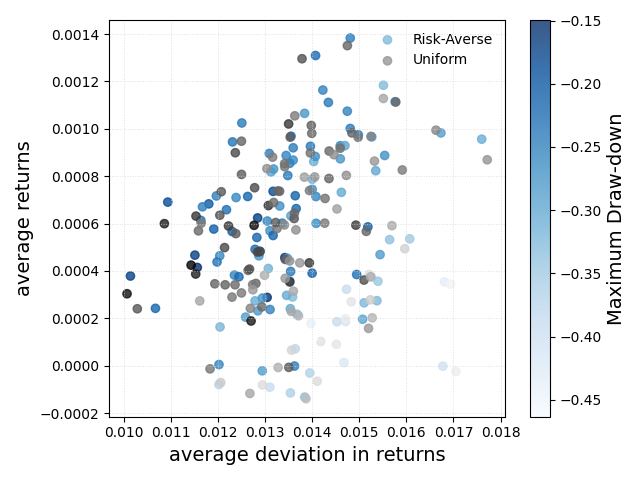
\includegraphics[width=\linewidth]{Images/ar_vs_ad_plot_HER_09mu.png}
    \caption{Average return vs. average deviation of returns for Risk Averse and and theoretically ideal Uniform portfolios.}
    \label{fig:pareto_plotU}
    \end{minipage}
    \vfill

    \begin{minipage}{0.45\textwidth}
    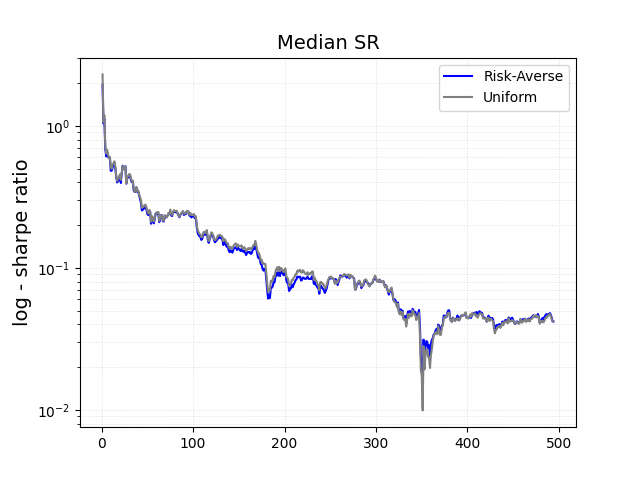
\includegraphics[width=\linewidth]{Images/mean_sr_HER_09mu.png}
    \caption{Sharpe ratio for Uniform \& Risk Averse portfolios.}
    \label{fig:sr_plot}
    \end{minipage}
\end{figure}

\begin{table}[H]
   \begin{minipage}{0.48\textwidth}
  % \centering
        \begin{tabular}{||l|r r||} % Example table
        \hline
        & Risk Averse & Uniform\\
        \hline
        max drawdown & -\textbf{0.273} & -0.280\\
        total return & 1.280 & 1.262 \\
        average return & 5.62e-4 & 5.37e-4 \\
        average return var. & 1.88e-4 & 1.86e-4 \\
        SR & 0.041 & 0.039 \\
        \hline
     \end{tabular}
  \end{minipage}
  \caption{Comparison of metrics' means $[\%]$}
          \label{tab:metrics_mean}
        \end{table}

  \begin{table}[H]
   \begin{minipage}{0.48\textwidth}
   % \centering
        \begin{tabular}{||l|r r||} % Example table
        \hline
        & Risk Averse & Uniform\\
        \hline
        max drawdown & -\textbf{0.259}& -0.271 \\
        total return & 1.269 & 1.265 \\
        average return & 5.68e-4 & 5.68e-4 \\
        average return var. & 1.84e-4 & 1.83e-4 \\
        SR & 0.042 & 0.042 \\
        \hline
        \end{tabular}
      \caption{Comparison of metrics' medians $[\%]$}
        \label{tab:metrics_median}
  \end{minipage}
\end{table}


\begin{figure}[H]
    \begin{minipage}{0.45\textwidth}
    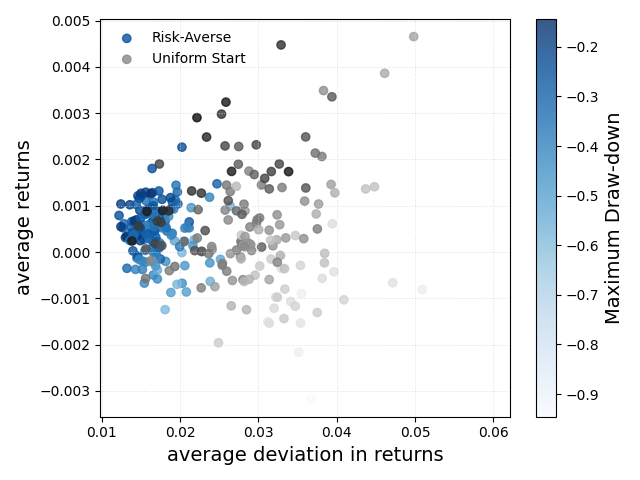
\includegraphics[width=\linewidth]{Images/ar_vs_ad_plot_HER_09_mu_se_uniformstart.png}
    \caption{Average return vs. average deviation of returns for Risk Averse and Uniform Start portfolios.}
    \label{fig:pareto_plotU-S}
    \end{minipage}
    \vfill

    \begin{minipage}{0.45\textwidth}
    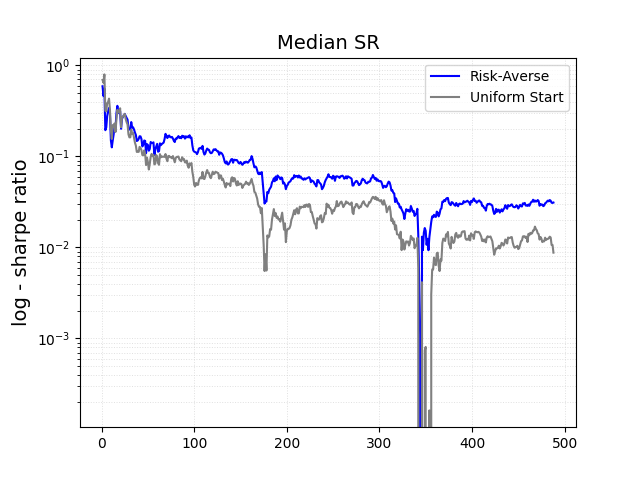
\includegraphics[width=\linewidth]{Images/median_sr_HER_09_mu_uniformstart.png}
    \caption{Sharpe ratio for Risk Averse \& Uniform Start portfolios.}
    \label{fig:sr_plotU-S}
    \end{minipage}
\end{figure}

\begin{table}[H]
    \begin{minipage}{0.48\textwidth}
        %\centering % Often good to center the table
        \begin{tabular}{||l|r r||} % Example table
        \hline
        & Risk Averse & Uniform Start\\
        \hline
        max drawdown & -\textbf{0.329} & -0.514\\
        total return & 1.21 & 1.222 \\
        average return & 4.58e-4 & 4.56e-4 \\
        average return var. & 2.94e-4 & 9.45e-4 \\
        SR & 0.027 & 0.015 \\
        \hline
        \end{tabular}
      \caption{Comparison of metrics' means $[\%]$} % <-- Use \captionof
        \label{tab:metrics_meanU-S}
    \end{minipage}
\end{table}

 \begin{table}[H]
    \begin{minipage}{0.48\textwidth}
      %  \centering % Often good to center the table
        \begin{tabular}{||l|r r||} % Example table
        \hline
        & Risk Averse & Uniform Start\\
        \hline
        max drawdown & -\textbf{0.316} & -0.499 \\
        total return & 1.18 & 0.915 \\
        average return & 5.17e-4 & 2.55e-4 \\
        average return var. & 2.75e-4 & 8.49e-4 \\
        SR & 0.031 & 0.009 \\
        \hline
        \end{tabular}
      \caption{Comparison of  metrics' medians $[\%]$}
        \label{tab:metrics_medianU-S}
    \end{minipage}
 \end{table}
 \end{figure} 
\section{Experimental Results}
\label{s:experiments}
This section reports a complete, paired comparison of the proposed policy with standard portfolio benchmarks, an ablation of its components, a sensitivity study of the user-set quantities, stress tests of the adaptive forgetting, and the behaviour on market windows outside the data used for design. All numbers are produced by the released code (Sec.~\ref{s:software}); every table and figure of this section is regenerated by a single script.

\subsection{\blt{Data and Protocol}} \label{s:data}
\emph{Universe.} From the S\&P~500 constituents we took the 100 stocks with the highest average daily return in 2021 and, among them, the 20 least pair-wise correlated ones: MRNA, COP, MOH, AXON, WST, EQT, AZO, DXCM, DELL, EXR, ENPH, BG, CRWD, EPAM, OXY, TGT, TSLA, CF, ANET, TSCO (Fig.~\ref{fig:corr_matrix}). The screen uses 2021 data only, i.e.\ it precedes the test period, but it is a screen on past performance and we return to its consequences in Sec.~\ref{s:regimes}. Daily simple returns are computed from dividend- and split-adjusted closing prices (Yahoo Finance).

\emph{Portfolios.} We draw 200 portfolios of 8--12 stocks uniformly at random from the universe (fixed seed). Every strategy, benchmark and ablation is run on exactly the same portfolios and the same days, so that all comparisons are paired.

\emph{Time line.} Each portfolio uses 750 trading days, 4 November 2022 -- 31 October 2025: the first $\bar t=125$ days build the optimal prior (Sec.~\ref{s:prior}), the next 125 days feed the structure estimation (Sec.~\ref{s:SE}), and the remaining 500 days, 3 November 2023 -- 31 October 2025, are the test period on which all metrics are computed. The hyperparameters $\mu,\alpha_0,\beta_0$ were fixed by a $2^k$ design on 2021--2022 data, which does not overlap the test period.

\emph{Transaction costs.} All strategies pay a proportional cost of $0.2\%$ of the traded value, $c_t = 0.002\sum_i |a_{i,t}-\tilde a_{i,t-1}|$, where $\tilde a_{t-1}$ are the previous weights after the drift caused by $y_{t-1}$, i.e.\ the actual trade. Every strategy starts from the uniform allocation. Wealth evolves as $W_{t+1}=W_t(1+a_t^\top y_t)(1-c_t)$. The same simulator is used for all strategies.

\emph{Metrics.} Total return $W_{500}/W_0$; annualised return and volatility; annualised Sharpe ratio $\sqrt{252}\,\bar r/\hat\sigma_r$ of daily net returns; maximum drawdown; Calmar ratio (annualised return over maximum drawdown); mean daily turnover $\sum_i|a_{i,t}-\tilde a_{i,t-1}|$; and the total cost paid.

\emph{Statistics.} Because every strategy is evaluated on the same portfolios, differences are tested with the Wilcoxon signed-rank test across the 200 (or 100) portfolios, complemented by a bootstrap 95\% confidence interval of the mean difference and the fraction of portfolios in which the proposed policy is better (win rate).

\subsection{\blt{Benchmarks}} \label{s:benchmarks}
\begin{itemize}\setlength{\itemsep}{1pt}
\item \emph{Equal-weight, rebalanced} to $1/N$ every day (pays costs) and \emph{equal-weight buy \& hold} (pays nothing after the initial allocation; this is the ``Uniform Start'' policy of the earlier version of this paper).
\item \emph{Inverse volatility}: $a_i\propto 1/\hat\sigma_i$ on a 60-day window.
\item \emph{Minimum variance} and \emph{mean-variance} (Markowitz, risk aversion 5) with long-only weights, Ledoit--Wolf shrinkage covariance, rolling windows of 120 and 250 days; mean-variance also in a \emph{cost-aware} version that penalises the trade from $\tilde a_{t-1}$ with the same $\mat{D}$ as our policy.
\item \emph{ARX-conditional mean-variance}: the same regressors $z_t$ selected by our structure estimation, but a rolling ridge regression as the predictor and a long-only mean-variance optimiser with the risk aversion equal to the $\omega^*$ used by our policy. It isolates the effect of the Bayesian learning and of the FPD-derived loss from the effect of the information in $z_t$.
\item \emph{S\&P~500}: buy and hold of the SPY exchange-traded fund (total return) over the same test days. It is a different, much larger, asset universe and is shown because it is the benchmark practitioners compare with.
\end{itemize}

\subsection{\blt{Ablations}} \label{s:ablations}
Each ablation removes or replaces one component of the policy and keeps everything else identical (same prior, regressors, portfolios, days):
\emph{no forgetting} (plain Bayesian update, $\alpha=0$, $\beta=1$); \emph{exponential forgetting} $0.99$; \emph{risk-neutral loss} (the FPD risk term with $\omega^*$ removed, only expected return and cost remain); \emph{no structure estimation} (all candidate regressors kept); \emph{flat prior} ($\mat{V}_0=10^{-6}\mat{I}$, $\Delta_0=\rho+2$) instead of the optimal prior; \emph{receding horizon} $h=5$ instead of $h=1$ with loss-to-go propagation; \emph{Thompson sampling} of $\theta$ in the design; and the constrained-QP solver of Sec.~\ref{s:optimization} versus the \emph{softmax heuristic} (Sec.~\ref{s:solver_note}).

\subsection{\blt{A Note on the Optimiser}} \label{s:solver_note}
The inner projected-gradient loop of the SMALBE implementation used for the experiments in the earlier versions of this manuscript contained an indexing error that made the routine return its starting point, the softmax of the unconstrained LQR action $-\mat{H}_a^{-1}\mat{H}_s s_{t-1}$. The published tables therefore described this heuristic, not the constrained optimum. The error is corrected in the released code, the corrected routine agrees with an independent SLSQP solver to $10^{-11}$ in the objective on random instances (\texttt{tests/test\_solver.py}), and we report both versions below because their behaviour differs qualitatively: the heuristic keeps the weights within a few percent of uniform, the constrained optimum does not.

\subsection{\blt{End-to-End Algorithm}} \label{s:algorithm}
Algorithm~1 (Fig.~\ref{alg:pipeline}) summarises the complete procedure as implemented in the released code (function \texttt{bench.policy.run\_policy}). Table~\ref{tab:hyper} lists every user-set quantity.

\begin{figure}[ht!]
\begin{minipage}{\columnwidth}
\noindent\rule{\linewidth}{0.6pt}\par\vspace{2pt}
\noindent\textbf{Algorithm 1} Bayesian adaptive portfolio optimisation\par
\noindent\rule{\linewidth}{0.4pt}\par\vspace{2pt}
\noindent\textbf{Input:} returns $y_t\in\mathbb{R}^N$, candidate regressors $\bar{z}_t\in\mathbb{R}^{\bar\rho}$, cost matrix $\mat{D}$, prior weights $(\alpha_0,\beta_0)$, shrinkage $\mu$, warm-up lengths $\bar{t}$, $T$.\\[2pt]
\noindent\emph{Off-line (days $1\ldots T$)}
\begin{enumerate}\setlength{\itemsep}{0pt}
\item Collect $\tilde{\mat{V}}_{\bar t}=\sum_{\tau\le\bar t}(y_\tau^\top,\bar z_\tau^\top)^\top(y_\tau^\top,\bar z_\tau^\top)$; solve the scalar equation of Sec.~\ref{s:prior} for $\Delta_0$; form $(\mat{V}_0,\mat{G}_0)$.
\item Accumulate $\mat{V}_T=\mat{V}_0+\sum_{\bar t<\tau\le T}(\cdot)(\cdot)^\top$; run the genetic algorithm of Sec.~\ref{s:SE} on $\ln l(u)$ \eqref{e:loglikelihoodk}; keep the regressors $z_t\subset\bar z_t$ of the maximiser $u^*$; restrict $\mat{V}_0$ to $(y_t,z_t)$ and recompute its square root $\mat{G}_0$.
\item Set $\mat{G}_T=\mat{G}_0$, $\Delta_T=\Delta_0$, $a_T=\mathbf{1}/N$, $\mat{H}_T=\epsilon\mat{I}$.
\end{enumerate}
\noindent\emph{On-line (each trading day $t>T$)}
\begin{enumerate}\setlength{\itemsep}{0pt}\setcounter{enumi}{3}
\item \textbf{Predict:} $\hat{\mat{P}}=\mat{G}_{zy}^\top\mat{G}_{z}^{-\top}$, $\hat y_t=\hat{\mat{P}}^\top z_t$, $\hat{\mat{\Sigma}}=\mat{G}_y\mat{G}_y^\top/\Delta_{t-1}$ \eqref{e:leastsquaresPwithG}.
\item \textbf{Elicit risk weight:} $\omega^*=\arg\min_{\omega>0}$ of \eqref{e:idealbehaviourminomega} given $\mat{D}$, $\hat{\mat{\Sigma}}$, $a_{t-1}$; build $\mat{Q}_{t-1}$ \eqref{e:lossmatrixQdefinition}.
\item \textbf{Design:} one Riccati step of Sec.~\ref{s:optimization} from $\mat{H}_{t-1}$ gives $(\mat{H}_a,\mat{H}_s)$; solve the constrained QP $\min_{a\in\Omega_{BE}}\|\mat{H}_a a+\mat{H}_s s_{t-1}\|^2$ (SMALBE, or any simplex-QP solver); output $a_t$.
\item \textbf{Trade} to $a_t$, pay $\mat{D}$-proportional costs, observe $y_t$.
\item \textbf{Learn:} minimise the forgetting criterion $F(\alpha,\beta,\gamma)$ of Sec.~\ref{s:forgetting} on the simplex (Nelder--Mead in the softmax parametrisation); update $\mat{G}_t$ by the orthogonal rotation of Sec.~\ref{s:forgetting} and $\Delta_t=(\alpha^*+\beta^*)\Delta_{t-1}+\beta^*+\gamma^*\Delta_0$.
\item \textbf{Propagate loss-to-go:} $\mat{H}_t=\phi^*\mat{H}_{t-1}+(1-\phi^*)\mat{H}_t^{\rm new}$ with $\phi^*$ minimising the KLD criterion of Sec.~\ref{s:optimization}.
\end{enumerate}
\noindent\rule{\linewidth}{0.6pt}
\end{minipage}
\caption{The complete procedure (Algorithm 1); step numbers refer to the released implementation.}
\label{alg:pipeline}
\end{figure}

\begin{table}[ht!]
\footnotesize
\setlength{\tabcolsep}{3pt}
\renewcommand{\arraystretch}{1.1}
\begin{tabular}{@{}l>{\raggedright\arraybackslash}p{0.40\columnwidth}>{\raggedright\arraybackslash}p{0.32\columnwidth}@{}}
\hline
quantity & role & value \\
\hline
$\mu$ & prior shrinkage, Sec.~\ref{s:prior} & 0.9 \\
$\alpha_0,\beta_0$ & prior forgetting weights, Sec.~\ref{s:forgetting} & 0.09, 0.5 \\
$\phi_0$ & prior weight of loss-to-go mixing & 0.1 \\
$\bar t$, $T$ & prior / structure warm-up [days] & 125, 125 \\
$h$ & receding horizon & 1 \\
$\mat{D}$ & transaction cost per unit traded & $0.002\,\mat{I}$ \\
$\bar z_t$ & candidate regressors & 10 lags, 3 EMA differences, 3 sines, intercept \\
GA & batch, $p_{mut}$, $\alpha_{decay}$, iterations & 8, 0.5, 0.992, 500 \\
$\omega_{\max}$ & upper bound of the risk-weight search & $10^3$ \\
\hline
\end{tabular}
\caption{All user-set quantities of the experiments. $\mu$, $\alpha_0$, $\beta_0$ were chosen by a $2^k$ design on 2021--2022 data, disjoint from the test period; the remaining values are conventional defaults that were not tuned.}
\label{tab:hyper}
\end{table}


%% Results text for the 2023--2025 window. Numbers from code/results/bench (200 portfolios, 100 for ablations).
\subsection{\blt{Results on the 2023--2025 Test Period}} \label{s:results}
Table~\ref{tab:bench_mean} reports the means over the 200 portfolios, Table~\ref{tab:bench_paired} the paired tests, Fig.~\ref{fig:bench_wealth} the median wealth paths and Fig.~\ref{fig:bench_sharpe} the distribution of the annualised Sharpe ratio.

\emph{The constrained-QP policy.} With the corrected optimiser the Risk-Averse policy (RA) has an annualised Sharpe ratio of $0.34$ and a total return of $1.11$, against $0.66$ and $1.27$ for the daily rebalanced equal-weight portfolio and $0.77$ and $1.36$ for equal-weight buy and hold. The differences are significant on every portfolio-level test (Wilcoxon $p<0.001$, RA better in 26\% and 20\% of the portfolios, respectively). The cause is visible in the last two columns: RA trades $15\%$ of the portfolio value per day and pays $15\%$ of the initial wealth in transaction costs over the two years, ten times more than the rebalanced equal-weight portfolio. Its gross performance (before costs) is comparable to the equal-weight benchmarks; it is the turnover that is not. RA does deliver what its name promises on one axis: its maximum drawdown ($-25.5\%$) is smaller than that of both equal-weight portfolios and much smaller than that of every mean-variance variant ($-40\%$ to $-42\%$), and its volatility is the lowest of the non-min-variance strategies. The only min-variance portfolio it does not beat on drawdown uses a 250-day window.

\emph{Why the turnover is high.} The risk weight $\omega^*$ of Sec.~\ref{s:FPD} is the minimiser of \eqref{e:idealbehaviourminomega} over $\omega>0$; in every one of the $10^5$ decision steps of the experiment the result is the upper bound of the search interval, $\omega_{\max}=10^3$. The necessary condition for an extreme stated in Sec.~\ref{s:FPD} is a sum of two terms that are positive for $\mat{D}\succ0$, $\hat{\mat{\Sigma}}\succeq0$ and $\omega>0$, so it has no root; the implementation minimises its left-hand side, which decreases monotonically in $\omega$, and the elicitation reduces to ``as risk-averse as allowed''. Sec.~\ref{s:sensitivity} treats $\omega_{\max}$ as the user-set quantity it effectively is. With $\omega=10^3$ the variance term $\tfrac{1}{2}\omega^2 a^\top\hat{\mat{\Sigma}}a$ in \eqref{e:lossmatrixQdefinition} is four orders of magnitude larger than the transaction-cost term $(a_t-a_{t-1})^\top\mat{D}(a_t-a_{t-1})$, so the cost is effectively not in the loss, and the policy re-optimises the minimum-variance-like allocation from scratch every day on a covariance estimate that is itself updated with heavy forgetting (Sec.~\ref{s:ablation_results}). The sensitivity study in Sec.~\ref{s:sensitivity} caps $\omega_{\max}$ and confirms this reading. This is also the mechanism behind the small drawdowns.

\emph{The legacy (softmax) policy.} The policy that produced the tables of the earlier version of this paper keeps the weights within a few percent of uniform (mean daily turnover $2.9\%$). Under the common cost model it is statistically indistinguishable from the rebalanced equal-weight portfolio in return and loses to it slightly but consistently in Sharpe ratio ($-0.03$, $p<0.001$, better in 1\% of the portfolios); it beats the min-variance and 120-day mean-variance portfolios in Sharpe ratio and all mean-variance portfolios in drawdown. Our earlier claim of outperforming the uniform portfolio rested on charging the uniform portfolio no costs and on the heuristic's near-uniform weights; it does not survive a paired test with identical cost treatment.

\emph{Classical benchmarks.} Plain mean-variance on a 250-day window has the highest return among the stock-universe strategies ($1.57$) at the price of a $-40\%$ maximum drawdown and a $37\%$ annualised volatility; its cost-aware variant halves the turnover of the 120-day version without changing the picture. The ARX-conditional mean-variance, which feeds the same regressors selected by our structure estimation into a ridge regression and a Markowitz optimiser with the same risk aversion $\omega^*$, loses money ($0.73$): the point forecasts of daily returns from these regressors are not tradeable through a classical optimiser, and the Bayesian learning with the FPD loss is what keeps RA from doing the same (RA beats it in $99.5\%$ of the portfolios). The S\&P~500 over the same days returned $1.62$ with a Sharpe ratio of $1.58$ and a drawdown of $-19\%$; no strategy on this 20-stock universe approaches it, including equal-weight buy and hold, which says more about the universe selected by the 2021 screen than about any allocation rule. We therefore do not claim to beat the index.

\begin{figure}[ht!]\centering
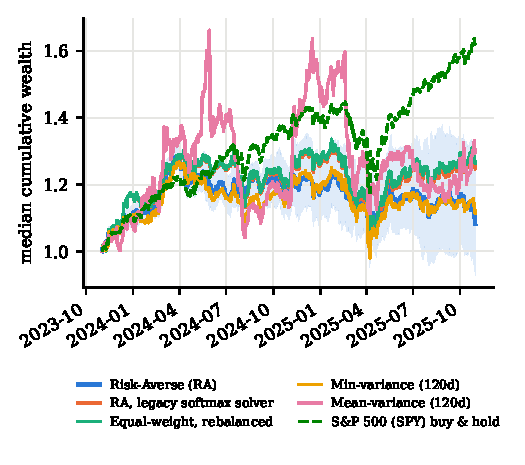
\includegraphics[width=0.48\textwidth]{Images/bench_wealth.pdf}
\caption{Median cumulative wealth over the 200 portfolios (band: interquartile range of RA). S\&P~500 is the same for all portfolios.}
\label{fig:bench_wealth}
\end{figure}
\begin{figure}[ht!]\centering
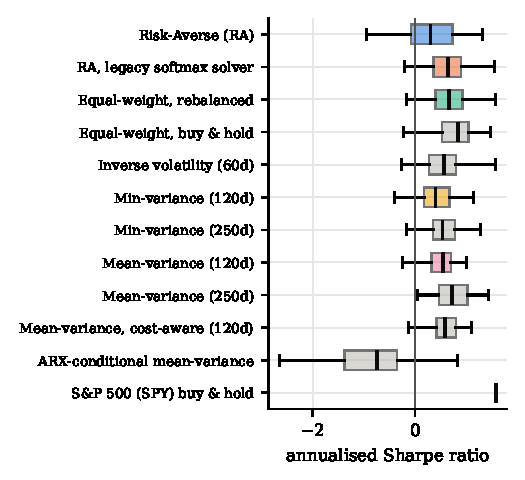
\includegraphics[width=0.48\textwidth]{Images/bench_sharpe.pdf}
\caption{Annualised Sharpe ratio across the 200 portfolios (boxes: quartiles, whiskers: 1.5 IQR).}
\label{fig:bench_sharpe}
\end{figure}

\subsection{\blt{Ablation Study}} \label{s:ablation_results}
Table~\ref{tab:ablation} and Fig.~\ref{fig:bench_ablation} isolate the components on 100 portfolios.
\begin{itemize}\setlength{\itemsep}{1pt}
\item \emph{Optimiser.} The corrected SMALBE of Sec.~\ref{s:optimization} and the SLSQP reference give identical allocations (maximum weight difference $3\cdot10^{-7}$), so the results do not depend on the QP solver; the softmax heuristic is a different policy (Sec.~\ref{s:results}).
\item \emph{Risk term.} Removing the FPD risk term (risk-neutral quadratic loss) is catastrophic: the policy chases the point forecast, turns the portfolio over $1.5$ times per day and loses $72\%$. The same happens with Thompson sampling of $\theta$ in the design ($-56\%$) and without structure estimation ($-49\%$): the parameter uncertainty of a 137-regressor model, or a sampled parameter, produces forecasts that the loss then trusts. The FPD risk term, the structure estimation and the point estimate are what make the daily return forecasts usable at all.
\item \emph{Forgetting.} Replacing the data-based forgetting by a plain Bayesian update changes nothing measurable (Sharpe $+0.04$, $p=0.13$); exponential forgetting $0.99$ is worse ($-0.22$, $p<0.001$). The median weights in Fig.~\ref{fig:bench_forgetting} explain why: the optimiser keeps $\gamma$, the weight of the prior, between $0.5$ and $0.8$ on almost every day, so the statistic is pulled more than half-way back to $\mat{V}_0$ daily and the model never moves far from the prior fitted on the first 125 days. The mechanism the forgetting was designed for is visible at the April 2025 tariff shock (shaded), where $\beta$ drops to zero and $\gamma$ rises, i.e.\ the outlying days are discarded; but on ordinary days the same mechanism discards most of the data as well.
\item \emph{Prior.} The flat prior gives the best numbers of all RA variants (Sharpe $0.72$, total return $1.30$, turnover $1.6\%$), but for a trivial reason: its allocations coincide with the rebalanced equal-weight portfolio to three decimals in every metric. With $\mat{V}_0=10^{-6}\mat{I}$ the forgetting pulls the statistic back to an isotropic covariance and to zero forecasts every day, and the constrained minimiser of a quadratic loss with $\hat{\mat{\Sigma}}\propto\mat{I}$ and $\hat y=0$ is $1/N$. The optimal prior of Sec.~\ref{s:prior} with $\mu=0.9$ is worth $\mu/(1-\mu)=9$ times the 125 days it is built from, i.e.\ 1125 days of pseudo-data; the sensitivity study (Sec.~\ref{s:sensitivity}) shows that $\mu=0.7$, which keeps fewer regressors and a weaker prior, is better than $0.9$, and that the forgetting prior $(\alpha_0,\beta_0)$ changes the forgetting weights but not the result.
\item \emph{Horizon.} The receding horizon $h=5$ without loss-to-go propagation gives the same allocations as $h=1$ with propagation (maximum weight difference $7\cdot10^{-6}$). At $\omega=10^3$ the one-step quadratic loss dominates the loss-to-go by orders of magnitude and the multi-step design is inactive.
\end{itemize}
\begin{figure}[ht!]\centering
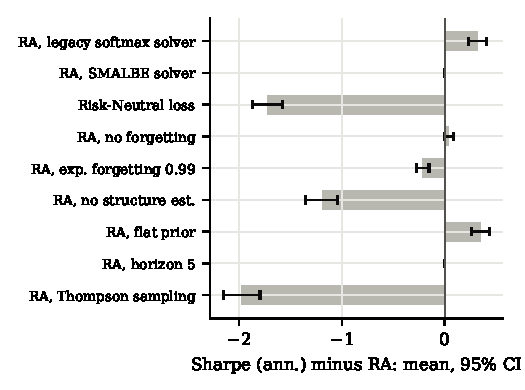
\includegraphics[width=0.48\textwidth]{Images/bench_ablation.pdf}
\caption{Annualised Sharpe ratio of each ablation minus that of the full Risk-Averse policy, paired over 100 portfolios (mean and bootstrap 95\% CI).}
\label{fig:bench_ablation}
\end{figure}
\begin{figure}[ht!]\centering
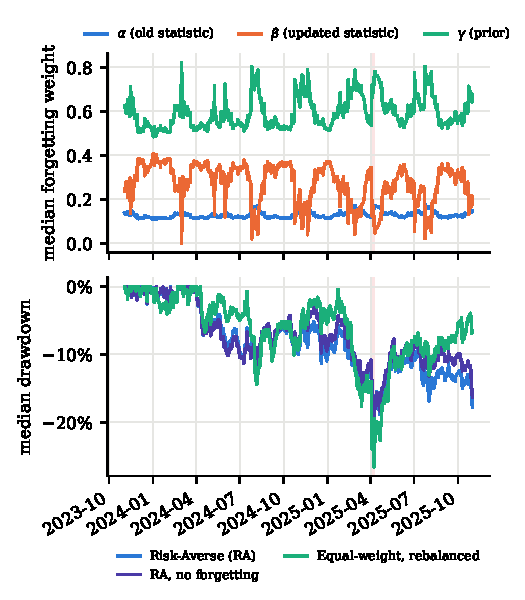
\includegraphics[width=0.48\textwidth]{Images/bench_forgetting.pdf}
\caption{Top: median optimal forgetting weights over the 200 portfolios. Bottom: median drawdown of RA, RA without forgetting and the rebalanced equal-weight portfolio; shaded: the tariff shock of 2--9 April 2025.}
\label{fig:bench_forgetting}
\end{figure}

\subsection{\blt{Stress Tests: Outliers and Parameter Changes}} \label{s:stress}
Fig.~\ref{fig:stress_synthetic} uses ARX data with known parameters (4 assets, 6 regressors, 700 days), two one-day crashes of $-12\%$ on all assets (days 300 and 450) and a sign flip of all regression coefficients at day 550. Three learners see identical data and start from the same optimal prior. On the crash days the data-based forgetting sets $\beta=0$ and $\gamma\approx1$: the outlier is discarded and the statistic reverts to the prior, and the estimation error does not move, whereas both other learners absorb the outlier (visible as a jump of the error after day 300 for the no-forgetting learner). This is the robustness to black-swan observations claimed in Sec.~\ref{s:forgetting}, and it holds. The same figure shows the price: during the stationary phase the optimal forgetting keeps the estimation error at its prior level ($0.72$) while the other learners improve to $0.5$, and after the parameter change it does not re-learn (the weights return immediately to their prior values, $\gamma\approx0.43$) while exponential forgetting halves the error within 150 days. Table~\ref{tab:ablation} showed the corresponding market result: no forgetting is at least as good. In its present form the mechanism therefore protects against outliers but not against slow or abrupt drift, and it does so by not learning; a forgetting prior $(\alpha_0,\beta_0,\gamma_0)$ that places less mass on $\gamma$ (Sec.~\ref{s:sensitivity}) is the obvious knob.
\begin{figure}[ht!]\centering
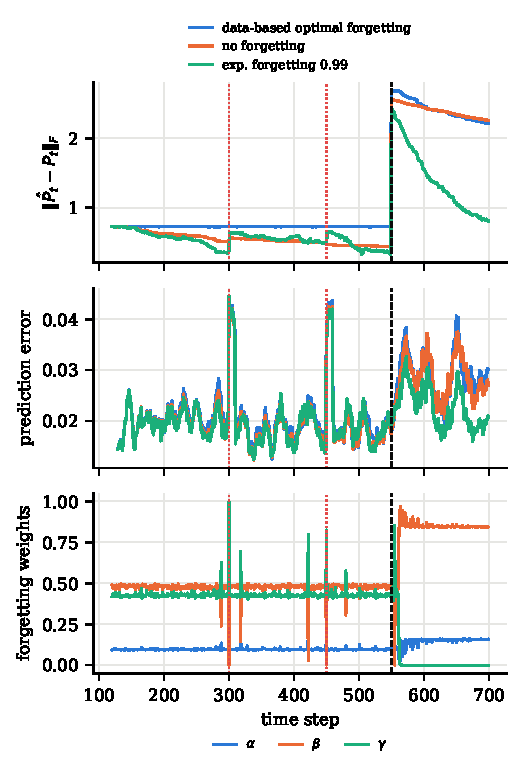
\includegraphics[width=0.48\textwidth]{Images/stress_synthetic.pdf}
\caption{Synthetic stress test. Top: parameter estimation error; middle: one-step prediction error (10-day mean); bottom: the optimal forgetting weights. Dotted: one-day crashes; dashed: change of all regression coefficients.}
\label{fig:stress_synthetic}
\end{figure}


\begin{table*}[ht!]
\centering
\footnotesize
\setlength{\tabcolsep}{4pt}
\begin{tabular}{lrrrrrrrr}
\hline
strategy & total return & ann. return & ann. vol. & Sharpe (ann.) & max DD & Calmar & turnover/day & cost paid \\
\hline
Risk-Averse (RA) & 1.114 & 5.0\% & 19.2\% & 0.34 & -25.5\% & 0.33 & 14.9\% & 14.9\% \\
RA, legacy softmax solver & 1.257 & 11.9\% & 21.0\% & 0.63 & -27.4\% & 0.47 & 2.9\% & 2.9\% \\
Equal-weight, rebalanced & 1.273 & 12.6\% & 20.9\% & 0.66 & -27.1\% & 0.50 & 1.6\% & 1.6\% \\
Equal-weight, buy \& hold & 1.357 & 16.3\% & 22.1\% & 0.77 & -28.8\% & 0.60 & 0.0\% & 0.0\% \\
Inverse volatility (60d) & 1.198 & 9.3\% & 19.0\% & 0.55 & -26.4\% & 0.39 & 2.3\% & 2.3\% \\
Min-variance (120d) & 1.128 & 6.0\% & 17.7\% & 0.41 & -24.6\% & 0.30 & 2.8\% & 2.8\% \\
Min-variance (250d) & 1.181 & 8.6\% & 17.3\% & 0.56 & -23.0\% & 0.43 & 2.0\% & 2.0\% \\
Mean-variance (120d) & 1.277 & 12.4\% & 37.2\% & 0.47 & -41.6\% & 0.33 & 15.3\% & 15.3\% \\
Mean-variance (250d) & 1.567 & 24.0\% & 37.0\% & 0.69 & -39.8\% & 0.67 & 8.6\% & 8.6\% \\
Mean-variance, cost-aware (120d) & 1.362 & 16.1\% & 36.2\% & 0.56 & -41.8\% & 0.42 & 1.1\% & 1.1\% \\
ARX-conditional mean-variance & 0.732 & -15.2\% & 18.7\% & -0.83 & -40.6\% & -0.33 & 43.6\% & 43.6\% \\
S\&P 500 (SPY) buy \& hold & 1.624 & 27.7\% & 16.3\% & 1.58 & -18.8\% & 1.48 & -- & -- \\
\hline
\end{tabular}
\caption{Benchmark comparison on the 500 test days 2023-11-03 to 2025-10-31, all strategies on the same random 8--12 stock portfolios, 0.2\% proportional transaction cost (mean over 200 portfolios).}
\label{tab:bench_mean}
\end{table*}

\begin{table*}[ht!]
\centering
\footnotesize
\setlength{\tabcolsep}{4pt}
\begin{tabular}{lrrrrrrrr}
\hline
benchmark & $\Delta$Sharpe & 95\% CI & $p$ & win rate & $\Delta$max DD & $p$ & $\Delta$total ret. & $p$ \\
\hline
RA, legacy softmax solver & -0.29 & [-0.35, -0.22] & $<$0.001 & 28\% & +2.0\% & $<$0.001 & -0.143 & $<$0.001 \\
Equal-weight, rebalanced & -0.32 & [-0.38, -0.26] & $<$0.001 & 26\% & +1.7\% & 0.002 & -0.159 & $<$0.001 \\
Equal-weight, buy \& hold & -0.43 & [-0.49, -0.37] & $<$0.001 & 20\% & +3.3\% & $<$0.001 & -0.243 & $<$0.001 \\
Inverse volatility (60d) & -0.21 & [-0.27, -0.15] & $<$0.001 & 30\% & +0.9\% & 0.029 & -0.084 & $<$0.001 \\
Min-variance (120d) & -0.07 & [-0.13, -0.02] & 0.008 & 44\% & -0.9\% & 0.152 & -0.014 & 0.089 \\
Min-variance (250d) & -0.22 & [-0.27, -0.16] & $<$0.001 & 34\% & -2.5\% & $<$0.001 & -0.067 & $<$0.001 \\
Mean-variance (120d) & -0.13 & [-0.20, -0.06] & $<$0.001 & 38\% & +16.1\% & $<$0.001 & -0.164 & $<$0.001 \\
Mean-variance (250d) & -0.35 & [-0.42, -0.27] & $<$0.001 & 24\% & +14.4\% & $<$0.001 & -0.454 & $<$0.001 \\
Mean-variance, cost-aware (120d) & -0.22 & [-0.28, -0.15] & $<$0.001 & 34\% & +16.4\% & $<$0.001 & -0.248 & $<$0.001 \\
ARX-conditional mean-variance & +1.17 & [+1.09, +1.25] & $<$0.001 & 100\% & +15.1\% & $<$0.001 & +0.382 & $<$0.001 \\
S\&P 500 (SPY) buy \& hold & -1.24 & [-1.32, -1.17] & $<$0.001 & 0\% & -6.7\% & $<$0.001 & -0.511 & $<$0.001 \\
\hline
\end{tabular}
\caption{Paired comparison of the Risk-Averse policy against every benchmark across portfolios: mean difference of the annualised Sharpe ratio with bootstrap 95\% CI, Wilcoxon signed-rank $p$-value, fraction of portfolios in which RA is better; the same for maximum drawdown (positive = smaller drawdown) and total return.}
\label{tab:bench_paired}
\end{table*}

\begin{table*}[ht!]
\centering
\footnotesize
\setlength{\tabcolsep}{4pt}
\begin{tabular}{lrrrrrrrr}
\hline
strategy & total return & ann. return & ann. vol. & Sharpe (ann.) & max DD & Calmar & turnover/day & cost paid \\
\hline
Risk-Averse (RA) & 1.126 & 5.6\% & 19.4\% & 0.37 & -25.5\% & 0.36 & 14.8\% & 14.8\% \\
RA, legacy softmax solver & 1.287 & 13.3\% & 21.0\% & 0.68 & -26.6\% & 0.53 & 2.9\% & 2.9\% \\
RA, SMALBE solver & 1.126 & 5.6\% & 19.4\% & 0.37 & -25.5\% & 0.36 & 14.8\% & 14.8\% \\
Risk-Neutral loss & 0.279 & -50.5\% & 47.5\% & -1.35 & -80.8\% & -0.60 & 155.4\% & 155.4\% \\
RA, no forgetting & 1.128 & 6.0\% & 17.9\% & 0.41 & -22.6\% & 0.37 & 14.8\% & 14.8\% \\
RA, exp. forgetting 0.99 & 1.032 & 1.3\% & 17.7\% & 0.15 & -26.1\% & 0.12 & 20.1\% & 20.1\% \\
RA, no structure est. & 0.512 & -31.6\% & 40.7\% & -0.82 & -64.2\% & -0.44 & 106.8\% & 106.8\% \\
RA, flat prior & 1.304 & 14.0\% & 21.0\% & 0.72 & -26.3\% & 0.57 & 1.6\% & 1.6\% \\
RA, horizon 5 & 1.126 & 5.6\% & 19.4\% & 0.37 & -25.5\% & 0.36 & 14.8\% & 14.8\% \\
RA, Thompson sampling & 0.442 & -37.1\% & 27.5\% & -1.60 & -63.4\% & -0.50 & 118.7\% & 118.7\% \\
\hline
\end{tabular}
\caption{Ablation study: each row removes or replaces one component of the Risk-Averse policy (mean over 100 portfolios).}
\label{tab:ablation}
\end{table*}

\begin{table*}[ht!]
\centering
\footnotesize
\setlength{\tabcolsep}{4pt}
\begin{tabular}{lrrrrrrrr}
\hline
benchmark & $\Delta$Sharpe & 95\% CI & $p$ & win rate & $\Delta$max DD & $p$ & $\Delta$total ret. & $p$ \\
\hline
RA, legacy softmax solver & -0.32 & [-0.40, -0.23] & $<$0.001 & 26\% & +1.1\% & 0.138 & -0.161 & $<$0.001 \\
RA, SMALBE solver & -0.00 & [-0.00, +0.00] & 0.853 & 51\% & +0.0\% & 0.931 & -0.000 & 0.915 \\
Risk-Neutral loss & +1.72 & [+1.58, +1.87] & $<$0.001 & 99\% & +55.4\% & $<$0.001 & +0.847 & $<$0.001 \\
RA, no forgetting & -0.04 & [-0.08, +0.00] & 0.130 & 47\% & -2.9\% & $<$0.001 & -0.002 & 0.667 \\
RA, exp. forgetting 0.99 & +0.21 & [+0.15, +0.28] & $<$0.001 & 74\% & +0.7\% & 0.077 & +0.095 & $<$0.001 \\
RA, no structure est. & +1.19 & [+1.04, +1.35] & $<$0.001 & 94\% & +38.8\% & $<$0.001 & +0.614 & $<$0.001 \\
RA, flat prior & -0.35 & [-0.43, -0.26] & $<$0.001 & 23\% & +0.9\% & 0.238 & -0.178 & $<$0.001 \\
RA, horizon 5 & -0.00 & [-0.00, +0.00] & 0.100 & 42\% & -0.0\% & 0.022 & -0.000 & 0.267 \\
RA, Thompson sampling & +1.97 & [+1.80, +2.15] & $<$0.001 & 100\% & +38.0\% & $<$0.001 & +0.684 & $<$0.001 \\
\hline
\end{tabular}
\caption{Paired comparison of the Risk-Averse policy against its ablations.}
\label{tab:ablation_paired}
\end{table*}


%% Hyperparameter sensitivity. Numbers from code/results/bench/{ra_mu*,ra_ab_*,ra_omega*} (100 portfolios).
\subsection{\blt{Hyperparameter Sensitivity}} \label{s:sensitivity}
Tables~\ref{tab:sensitivity} and \ref{tab:sensitivity_paired} vary, one at a time, the three user-set quantities that the $2^k$ design tuned and the bound $\omega_{\max}$ that Sec.~\ref{s:results} identified as the effective risk weight; 100 portfolios, everything else as in Table~\ref{tab:hyper}.

\emph{Prior shrinkage $\mu$.} Smaller $\mu$ means a weaker prior (worth $\mu/(1-\mu)$ times the 125 days it is built from) and, through the marginal likelihood, a sparser structure: the genetic algorithm keeps 15 of 137 regressors at $\mu=0.7$ against 57 at $\mu=0.9$ and 78 at $\mu=0.95$. $\mu=0.7$ improves the Sharpe ratio by $0.18$ ($p<0.001$, better in 79\% of the portfolios) and reduces the turnover from $15\%$ to $11\%$ per day; $\mu=0.95$ is worse. The value $0.9$ chosen on 2021--2022 data is therefore not the best value on 2023--2025, but the ranking against the benchmarks does not change: even $\mu=0.7$ stays below the equal-weight portfolio.

\emph{Forgetting prior $(\alpha_0,\beta_0)$.} The optimised forgetting weights follow their prior closely (median $\gamma$ of $0.68$, $0.57$, $0.12$ and $0.00$ for $\gamma_0=0.6$, $0.41$, $0.1$ and $0.05$), but none of the three alternatives changes any performance metric by more than $0.01$ in Sharpe ratio. Together with the ablation of Sec.~\ref{s:ablation_results} this shows that the data-based forgetting is inert on this data: what the model predicts is fixed by the prior and the structure, not by how the statistic is updated.

\emph{The risk weight.} Capping the search interval of $\omega^*$ exposes the mechanism of Sec.~\ref{s:results}. With $\omega_{\max}=1$ the residual-minimising search of the implementation returns the lower end of the interval ($\omega\approx10^{-5}$), the return term disappears from the loss, the optimal action is $a_t=a_{t-1}$, and the policy is the rebalanced equal-weight portfolio to three decimals. With $\omega_{\max}=10$ or $100$ (the search returns the bound) the return forecasts enter the loss with a weight that lets them dominate the variance term, the policy takes corner positions in single stocks, turns the portfolio over 1.6 and 0.9 times per day, and loses $73\%$ and $46\%$ of the capital, as the risk-neutral ablation does. The same happens with the three principled elicitations of $\omega$ we tried in place of the search bound (the $\omega$ that makes the KLD between the model and the ideal equal to $1/2$, the $\omega$ that makes the ideal's mean shift equal to the predicted return, and a fixed $\omega=40$; their $\omega$ lies between 27 and 91 in 80\% of the decision steps): they lose $63$--$65\%$ of the capital with a daily turnover of $1.3$. Only $\omega=10^3$, where the variance term dominates by two orders of magnitude and the forecasts are effectively ignored, gives a usable policy. The reason is the forecasts themselves. On the 500 test days of the first ten portfolios the one-step-ahead predictions $\hat y_t$ have a standard deviation of $0.0267$ against $0.0269$ for the realised returns, a correlation with them of $-0.01$ (per asset: $-0.01$), a sign accuracy of $49.7\%$, and a mean squared error twice that of predicting zero (\texttt{bench/forecast\_quality.py}). They are as large as the returns and carry no information, so any loss that takes them at face value trades on noise, and a large $\omega$ is the only setting in which the design does not. The elicitation of $\omega$ in Sec.~\ref{s:FPD}, whatever its analytical form, cannot repair this, and the practical conclusion is that the point forecast must be shrunk (or the design must integrate over the parameter uncertainty that the posterior provides) before it enters the loss.

\begin{table*}[ht!]
\centering
\footnotesize
\setlength{\tabcolsep}{4pt}
\begin{tabular}{lrrrrrrrr}
\hline
strategy & total return & ann. return & ann. vol. & Sharpe (ann.) & max DD & Calmar & turnover/day & cost paid \\
\hline
Risk-Averse (RA) & 1.126 & 5.6\% & 19.4\% & 0.37 & -25.5\% & 0.36 & 14.8\% & 14.8\% \\
RA, $\mu=0.5$ & 1.150 & 7.0\% & 18.4\% & 0.45 & -22.0\% & 0.42 & 16.9\% & 16.9\% \\
RA, $\mu=0.7$ & 1.190 & 8.8\% & 18.4\% & 0.55 & -21.5\% & 0.53 & 10.9\% & 10.9\% \\
RA, $\mu=0.95$ & 1.096 & 4.2\% & 19.7\% & 0.30 & -26.5\% & 0.25 & 18.4\% & 18.4\% \\
RA, $(\alpha_0,\beta_0)=(0.2,0.2)$ & 1.127 & 5.6\% & 19.4\% & 0.37 & -25.5\% & 0.36 & 14.8\% & 14.8\% \\
RA, $(\alpha_0,\beta_0)=(0.3,0.6)$ & 1.122 & 5.5\% & 19.0\% & 0.37 & -24.8\% & 0.37 & 14.9\% & 14.9\% \\
RA, $(\alpha_0,\beta_0)=(0.5,0.45)$ & 1.119 & 5.4\% & 18.8\% & 0.37 & -24.5\% & 0.35 & 15.2\% & 15.2\% \\
RA, $\omega_{\max}=1$ & 1.305 & 14.0\% & 21.0\% & 0.72 & -26.3\% & 0.57 & 1.6\% & 1.6\% \\
RA, $\omega_{\max}=10$ & 0.266 & -50.5\% & 38.7\% & -1.72 & -79.1\% & -0.63 & 159.7\% & 159.7\% \\
RA, $\omega_{\max}=100$ & 0.541 & -27.5\% & 23.3\% & -1.31 & -55.4\% & -0.48 & 92.4\% & 92.4\% \\
RA, $\omega$: unit KLD & 0.353 & -41.8\% & 29.5\% & -1.76 & -70.3\% & -0.58 & 132.2\% & 132.2\% \\
RA, $\omega$: match prediction & 0.367 & -40.4\% & 27.4\% & -1.82 & -68.6\% & -0.58 & 127.8\% & 127.8\% \\
RA, $\omega=40$ & 0.358 & -41.3\% & 28.4\% & -1.80 & -69.7\% & -0.58 & 131.5\% & 131.5\% \\
\hline
\end{tabular}
\caption{Sensitivity to the user-set hyperparameters (prior shrinkage $\mu$, prior forgetting weights) (mean over 100 portfolios).}
\label{tab:sensitivity}
\end{table*}

\begin{table*}[ht!]
\centering
\footnotesize
\setlength{\tabcolsep}{4pt}
\begin{tabular}{lrrrrrrrr}
\hline
benchmark & $\Delta$Sharpe & 95\% CI & $p$ & win rate & $\Delta$max DD & $p$ & $\Delta$total ret. & $p$ \\
\hline
RA, $\mu=0.5$ & -0.08 & [-0.13, -0.03] & 0.005 & 40\% & -3.5\% & $<$0.001 & -0.024 & 0.030 \\
RA, $\mu=0.7$ & -0.18 & [-0.23, -0.13] & $<$0.001 & 21\% & -3.9\% & $<$0.001 & -0.063 & $<$0.001 \\
RA, $\mu=0.95$ & +0.07 & [+0.02, +0.12] & 0.005 & 65\% & +1.1\% & 0.006 & +0.030 & 0.010 \\
RA, $(\alpha_0,\beta_0)=(0.2,0.2)$ & -0.00 & [-0.00, -0.00] & $<$0.001 & 36\% & +0.0\% & 0.201 & -0.001 & $<$0.001 \\
RA, $(\alpha_0,\beta_0)=(0.3,0.6)$ & -0.00 & [-0.02, +0.01] & 0.003 & 68\% & -0.7\% & 0.341 & +0.004 & 0.003 \\
RA, $(\alpha_0,\beta_0)=(0.5,0.45)$ & +0.00 & [-0.02, +0.02] & 0.570 & 53\% & -0.9\% & $<$0.001 & +0.007 & 0.196 \\
RA, $\omega_{\max}=1$ & -0.35 & [-0.44, -0.26] & $<$0.001 & 23\% & +0.9\% & 0.236 & -0.179 & $<$0.001 \\
RA, $\omega_{\max}=10$ & +2.09 & [+1.95, +2.23] & $<$0.001 & 99\% & +53.6\% & $<$0.001 & +0.860 & $<$0.001 \\
RA, $\omega_{\max}=100$ & +1.68 & [+1.60, +1.76] & $<$0.001 & 100\% & +29.9\% & $<$0.001 & +0.585 & $<$0.001 \\
RA, $\omega$: unit KLD & +2.13 & [+2.02, +2.24] & $<$0.001 & 99\% & +44.9\% & $<$0.001 & +0.773 & $<$0.001 \\
RA, $\omega$: match prediction & +2.19 & [+2.08, +2.30] & $<$0.001 & 100\% & +43.1\% & $<$0.001 & +0.759 & $<$0.001 \\
RA, $\omega=40$ & +2.17 & [+2.07, +2.28] & $<$0.001 & 100\% & +44.2\% & $<$0.001 & +0.768 & $<$0.001 \\
\hline
\end{tabular}
\caption{Paired comparison of the default hyperparameters against the alternatives.}
\label{tab:sensitivity_paired}
\end{table*}



%% Other market regimes and the out-of-sample window. Numbers from code/results/bench_{covid,bear2022,oos2026}.
\subsection{\blt{Other Market Regimes and an Out-of-Sample Window}} \label{s:regimes}
The 2023--2025 test period is a bull market. Table~\ref{tab:regimes} repeats the comparison, with the same universe, protocol, hyperparameters and 100 random portfolios per window, on three further 500-day windows: 2019--2020, which contains the COVID crash; 2021--2022, which contains the 2022 bear market; and September 2024 to September 2026, which lies almost entirely after the data used to design and tune the method and contains the live-test period of Sec.~\ref{s:live}. The 2019--2022 windows use the prices of the same 20 stocks before the 2021 screen that selected them, so they carry the selection bias of that screen (the stocks were chosen because they did well in 2021); the 2024--2026 window is free of it.

Three facts are stable across all four windows. (i) The corrected Risk-Averse policy has a lower Sharpe ratio than the rebalanced equal-weight portfolio in every window ($-0.2$ to $-0.8$, $p<0.001$), for the same reason as in Sec.~\ref{s:results}: it pays $11$--$15\%$ of its wealth in transaction costs per window. (ii) The legacy heuristic is the equal-weight portfolio plus $1\%$ of extra turnover: its Sharpe ratio is $0.02$ below that of the rebalanced equal-weight portfolio in every window, with a win rate of at most $4\%$. (iii) Against mean-variance the picture reverses with the regime: mean-variance made $4$--$7\times$ in 2019--2020 on the momentum of a few stocks and lost money in 2021--2022, whereas the Risk-Averse policy has a smaller drawdown than the 250-day mean-variance portfolio in $76$--$96\%$ of the portfolios in every window and a higher Sharpe ratio in the bear market ($+0.78$, $p<0.001$). In 2021--2022 both versions of the policy also beat the S\&P~500 in Sharpe ratio ($+0.53$ and $+0.72$), as does every low-turnover strategy on this universe; in the other windows the index is better. The out-of-sample window confirms the 2023--2025 ranking with no free parameter: equal-weight $1.06$, inverse volatility $0.91$, Risk-Averse $0.53$, S\&P~500 $1.16$.

\begin{table*}[ht!]
\centering
\footnotesize
\setlength{\tabcolsep}{4pt}
\begin{tabular}{lrrrrrrrrrrrr}
\hline
strategy & \multicolumn{3}{c}{2019-01 -- 2020-12} & \multicolumn{3}{c}{2021-01 -- 2022-12} & \multicolumn{3}{c}{2023-11 -- 2025-10} & \multicolumn{3}{c}{2024-09 -- 2026-09} \\
 & Sharpe & max DD & return & Sharpe & max DD & return & Sharpe & max DD & return & Sharpe & max DD & return \\
\hline
Risk-Averse (RA) & 0.71 & -40\% & 1.39 & 0.77 & -28\% & 1.37 & 0.34 & -25\% & 1.11 & 0.53 & -23\% & 1.20 \\
RA, legacy softmax solver & 1.46$^{*}$ & -37\% & 2.27 & 0.96$^{*}$ & -23\% & 1.55 & 0.63$^{*}$ & -27\% & 1.26 & 1.04$^{*}$ & -25\% & 1.55 \\
Equal-weight, rebalanced & 1.48$^{*}$ & -36\% & 2.29 & 0.98$^{*}$ & -23\% & 1.56 & 0.66$^{*}$ & -27\% & 1.27 & 1.06$^{*}$ & -25\% & 1.56 \\
Equal-weight, buy \& hold & 1.79$^{*}$ & -41\% & 3.75 & 0.92$^{*}$ & -23\% & 1.51 & 0.77$^{*}$ & -29\% & 1.36 & 1.01$^{*}$ & -26\% & 1.55 \\
Inverse volatility (60d) & 1.37$^{*}$ & -35\% & 1.99 & 1.06$^{*}$ & -23\% & 1.57 & 0.55$^{*}$ & -26\% & 1.20 & 0.91$^{*}$ & -25\% & 1.39 \\
Min-variance (250d) & 1.17$^{*}$ & -33\% & 1.70 & 1.01$^{*}$ & -24\% & 1.47 & 0.56$^{*}$ & -23\% & 1.18 & 0.67$^{*}$ & -21\% & 1.24 \\
Mean-variance (250d) & 1.66$^{*}$ & -44\% & 4.66 & -0.01$^{*}$ & -37\% & 0.90 & 0.69$^{*}$ & -40\% & 1.57 & 0.83$^{*}$ & -35\% & 1.85 \\
S\&P 500 (SPY) buy \& hold & 0.93$^{*}$ & -34\% & 1.49 & 0.23$^{*}$ & -24\% & 1.05 & 1.58$^{*}$ & -19\% & 1.62 & 1.16$^{*}$ & -19\% & 1.42 \\
\hline
\end{tabular}
\caption{Mean annualised Sharpe ratio, maximum drawdown and total return over 100 random portfolios (200 for the paper window) in four 500-day test windows: 2019--2020 contains the COVID crash, 2021--2022 the 2022 bear market, 2023--2025 is the window of the previous sections, 2024--2026 lies after the paper's data. Each window uses its own 250-day warm-up. $^{*}$: Sharpe ratio differs from that of the Risk-Averse policy at $p<0.01$ (paired Wilcoxon).}
\label{tab:regimes}
\end{table*}


\subsection{Live Test} \label{s:live}
\bl{We traded the policy with real money from 1 March to 15 April 2026 on a three-stock portfolio (Figs.~\ref{fig:cum_wealth_live}, \ref{fig:allocation_live}, Table~\ref{tab:live_metrics}). Over 32 trading days the policy returned $2.3\%$ against $2.2\%$ for the S\&P~500 and $5.6\%$ for the equal-weight portfolio, with the largest drawdown of the three. We keep the test because it demonstrates that the pipeline runs end-to-end on a broker feed, not as evidence of performance: 32 days cannot separate strategies whose daily returns differ by a fraction of a percent, and the 2024--2026 window above, which contains these dates, gives the same ranking on 100 portfolios.}


%% figures/table carried over verbatim from the previous version of the section
\begin{figure}[ht!]
    \begin{minipage}{0.45\textwidth}
    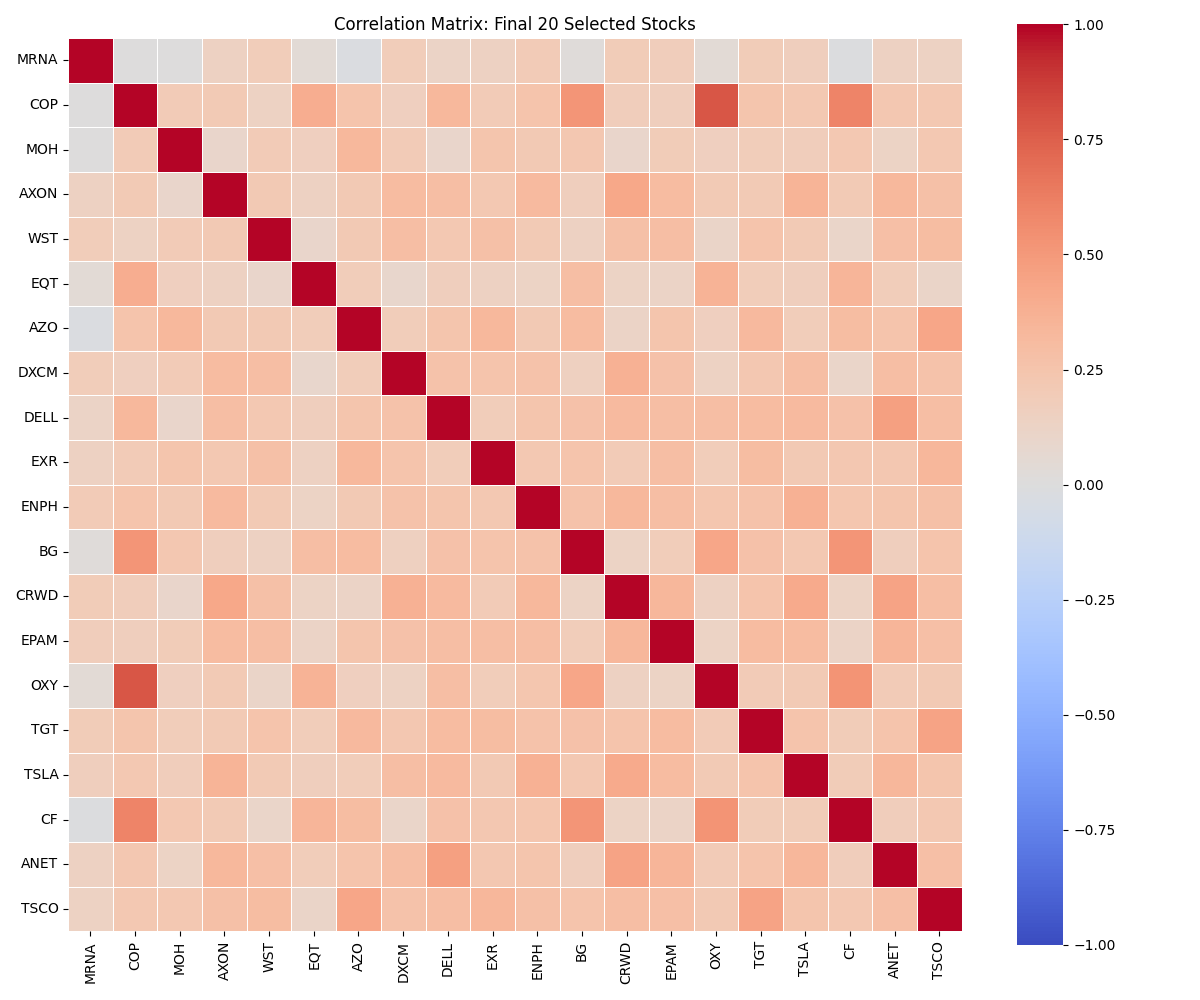
\includegraphics[width=\linewidth]{Images/selected_corr_matrix.png}
    \caption{Correlation matrix of the 20 selected stocks for our experiments.}
    \label{fig:corr_matrix}
    \end{minipage}
\end{figure}

\begin{figure}[ht!]
    \begin{minipage}{0.45\textwidth}
    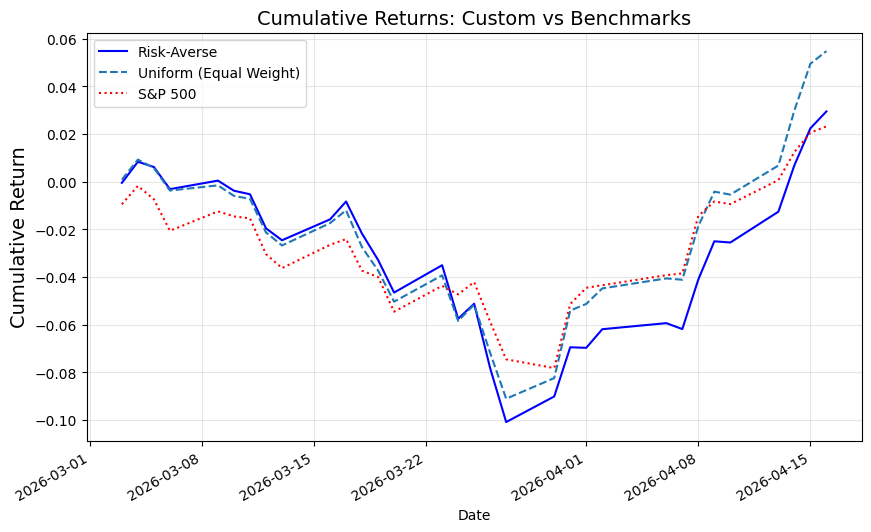
\includegraphics[width=\linewidth]{Images/live_returns.png}
    \caption{Returns comparison in live test. Risk Averse vs. Ideal Uniform portfolio vs. S\&P500 index benchmark.}
    \label{fig:cum_wealth_live}
    \end{minipage}
    \vfill

    \begin{minipage}{0.45\textwidth}
    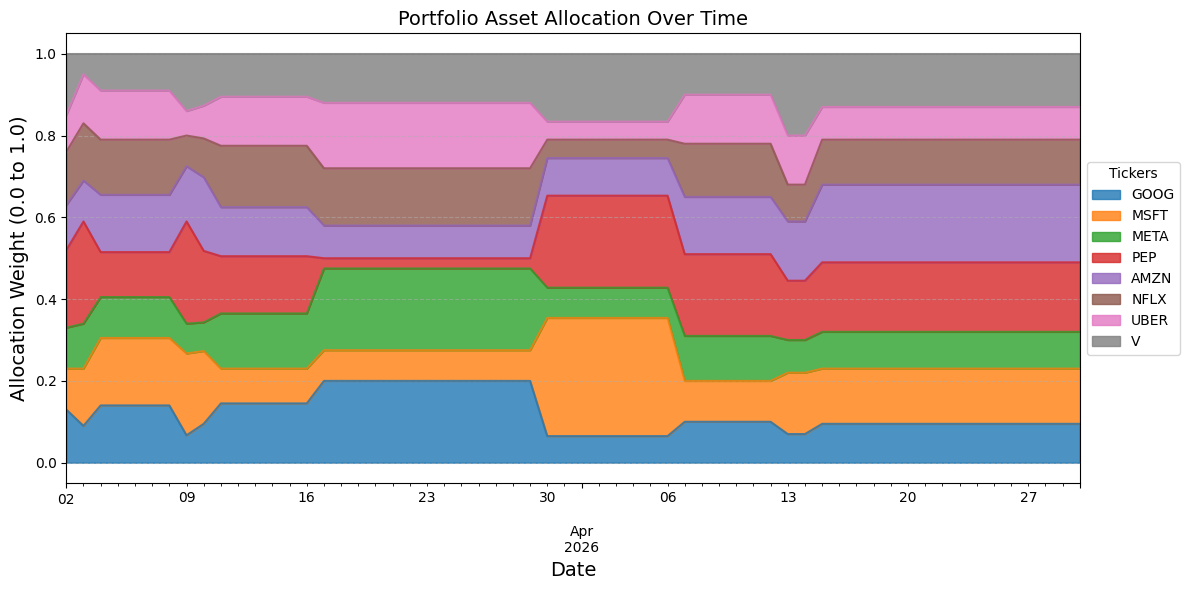
\includegraphics[width=\linewidth]{Images/live_allocation.png}
    \caption{Allocations of Risk Averse policy in live test.}
    \label{fig:allocation_live}
    \end{minipage}
\end{figure}

\begin{table}[ht!]
   \begin{minipage}{0.48\textwidth}
   % \centering
        \begin{tabular}{||l|r r r||} % Example table
        \hline
        & RA & U & S\&P500\\
        \hline
        max draw-down & -\textbf{0.108}& -0.099 & -0.077\\
        total return & \textbf{1.023} & 1.056 & 1.022\\
        SR & 0.074 & 0.133 & 0.069\\
        \hline
        \end{tabular}
      \caption{Comparison of live trading metrics.}
        \label{tab:live_metrics}
  \end{minipage}
\end{table}


\subsection{\blt{Computational Cost}} \label{s:runtime}
Table~\ref{tab:runtime} lists the cost of one portfolio on one core (Python/NumPy, no compiled code): the optimal prior and the 500-iteration genetic algorithm over $2^{137}$ structures take $2.6$\,s and keep 57 of 137 regressors on average; one trading day of the online loop (forgetting optimisation, Riccati step, constrained QP, loss-to-go propagation) takes $0.1$\,s. The whole study of this section, about 3000 portfolio-years, ran in under two hours on 20 cores.
\begin{table*}[ht!]
\centering
\small
\setlength{\tabcolsep}{4pt}
\begin{tabular}{lrrrr}
\hline
variant & regressors selected & setup [s] & time / step [s] & fallbacks \\
\hline
Risk-Averse (RA) & 57 / 137 & 2.6 & 0.10 & 0 \\
RA, legacy softmax solver & 57 / 137 & 2.6 & 0.09 & 0 \\
RA, SMALBE solver & 57 / 136 & 2.5 & 0.24 & 0 \\
Risk-Neutral loss & 57 / 136 & 2.6 & 0.09 & 0 \\
RA, no forgetting & 57 / 136 & 2.6 & 0.08 & 0 \\
RA, exp. forgetting 0.99 & 57 / 136 & 2.6 & 0.08 & 0 \\
RA, no structure est. & 136 / 136 & 0.0 & 0.37 & 0 \\
RA, flat prior & 131 / 136 & 6.7 & 0.23 & 0 \\
RA, horizon 5 & 57 / 136 & 2.8 & 0.04 & 0 \\
RA, Thompson sampling & 57 / 136 & 2.8 & 0.10 & 0 \\
\hline
\end{tabular}
\caption{Computational cost per portfolio (means): regressors kept by the structure estimation out of the full set, prior + structure estimation time, and wall time per trading day of the online loop (single core).}
\label{tab:runtime}
\end{table*}



\section{Conclusions} \label{s:conclusions}

\bl{The paper gives a complete, internally consistent solution of the adaptive portfolio-optimisation problem, from the choice of the prior to a numerically safe constrained design, and evaluates it with a paired protocol that any alternative can be plugged into. The evaluation does not confirm that the solution pays back in its present form: after transaction costs the policy is dominated by the equal-weight portfolio, while it does deliver smaller drawdowns than mean-variance allocation and rejects outlying observations as designed. The ablation and sensitivity studies locate the two elements responsible, the elicitation of the risk weight $\omega$, which has no interior optimum, and the strength of the optimal prior combined with the forgetting, which prevents the model from learning beyond its initial estimate. Both are local and are the first items of future work; the released code makes the corresponding experiments a matter of changing one line.}

An immediate enrichment concerns exploration that may significantly help the large investors influencing the market. The randomised nature of the FPD optimal policy is directly beneficial in this respect, as it naturally adds an adequate random component to poorly exciting actions, which would result from the standard LQR solution. 

The randomisation effect can be enhanced by the use of Thompson's sampling \cite{Rusetal:18}, which may additionally serve for off-line prediction of
the achieved quality even without closing the decision loop. It suffices to exploit the fact that the unknown parameter $\theta\in\Theta$ is described by the available PDF $p(\theta|\mathcal{D}^{\bar{t}})$. This allows: $\bullet$ sample
$\theta^{k} \sim p(\theta|\mathcal{D}^{\bar{t}})$; $\bullet$ perform the optimisation (LQR design) with this parameter; $\bullet$ use the gained sample of the final loss-to-go $v^{k}(s)$ for a (non)parametric estimate of its PDF, cf.\ \cite{KarJen:900078}.

The PDF gained in the off-line mode provides the mentioned prediction of the achievable quality. In online mode, it allows for robustifying the design, which makes the gained policy even more risk-aware.

The most promising advancement is the use of more general models. Mixture ratios, \cite{KarRum:21a}, are our favourite as they offer an efficient \bl{way to address} black swan events, \cite{bogle2008black}. It needs, however,  to reach solution completeness. It requires elaborating an efficient structure estimation, safe numerical implementation for mixed (continuous and discrete) modelled random variables, and the corresponding, inevitably approximate, dynamic programming, \cite{SiBarPowWunsch:04}.


\section*{Contribution, Competing Interest, Data and Software Access}
T. Proch\'{a}zka contributed to writing, reviewing, software, data handling and experiments. M.\ K\'{a}rn\'{y} provided  conceptualisation, and contributed to writing  and reviewing.

The authors have no known competing financial interests or personal relationships that could have appeared to influence the work reported in this paper.

\label{s:software} \bl{Public data were used only. The complete code, the data preparation and the scripts that regenerate every table and figure of Sec.~\ref{s:experiments} are available at \url{https://github.com/ProchTomas/ResearchProject}.}

\begin{thebibliography}{10}
\expandafter\ifx\csname url\endcsname\relax
  \def\url#1{\texttt{#1}}\fi
\expandafter\ifx\csname urlprefix\endcsname\relax\def\urlprefix{URL }\fi
\expandafter\ifx\csname href\endcsname\relax
  \def\href#1#2{#2} \def\path#1{#1}\fi

\bibitem{Pet:81}
V.~Peterka, {B}ayesian system identification, in: P.~Eykhoff (Ed.),
  Trends\,\&\,Progress in System Identification, 1981, pp. 239--304.

\bibitem{KarKul:88}
M.~K\'{a}rn\'{y}, R.~Kulhav\'{y}, Structure determination of regression-type
  models for adaptive prediction and control, in: J.~Spall (Ed.), {B}ayesian
  Analysis of Time Series and Dynamic Models, Marcel Dekker, 1988.

\bibitem{Kar:25a}
M.~K\'{a}rn\'{y}, Optimised conjugate prior for model structure estimation in
  the exponential family, Expert Systems with Applications 283 (2025) 127716.

\bibitem{Kul:93a}
R.~Kulhav{\'y}, Implementation of {B}ayesian parameter estimation in adaptive
  control and signal processing, The Statistician 42 (1993) 471--482.

\bibitem{AstWit:94}
K.~{A}str{\"{o}}m, B.~Wittenmark, Adaptive Control, Addison-Wesley, 1994.

\bibitem{Kar:19}
M.~K\'{a}rn\'{y}, Fully probabilistic design unifies and supports dynamic
  decision making under uncertainty, Inf. Sci. 509 (2020) 104--18.

\bibitem{dostal2009optimal}
Z.~Dost{\'a}l, Optimal Quadratic Programming Algorithms: With Applications to
  Variational Inequalities, Springer Optimization and Its Applications,
  Springer US, 2009.

\bibitem{haldurai2016study}
L.~Haldurai, T.~Madhubala, R.~Rajalakshmi, A study on genetic algorithm and its
  applications, Int. J. Comput. Sci. Eng 4~(10) (2016) 139--143.

\bibitem{BenLeaPue:25}
S.~Benati, M.~Leal, J.~Puerto, Bilevel portfolio optimization with ordered
  pricing models, Omega 133 (2025) 103274.
\newblock \href {https://doi.org/https://doi.org/10.1016/j.omega.2024.103274}
  {\path{doi:https://doi.org/10.1016/j.omega.2024.103274}}.

\bibitem{LiGaoShu:26}
B.~Li, Q.~Gao, Y.~Shu, Modeling of portfolio optimization with returns
  uncertainty and cross-efficiency evaluation, Omega 143 (2026) 103566.
\newblock \href {https://doi.org/https://doi.org/10.1016/j.omega.2026.103566}
  {\path{doi:https://doi.org/10.1016/j.omega.2026.103566}}.

\bibitem{LyuWuGuoGuChi:24}
B.~Lyu, B.~Wu, S.~Guo, J.-W. Gu, W.-K. Ching, Robust online portfolio
  optimization with cash flows, Omega 129 (2024) 103169.
\newblock \href {https://doi.org/https://doi.org/10.1016/j.omega.2024.103169}
  {\path{doi:https://doi.org/10.1016/j.omega.2024.103169}}.

\bibitem{michaud1989markowitz}
R.~Michaud, The {M}arkowitz optimization enigma: {I}s ‘optimized’optimal?,
  Financial analysts journal 45~(1) (1989) 31--42.

\bibitem{abbracciavento2025model}
F.~Abbracciavento, F.~Tappi, S.~Formentin, Model predictive control for
  multi-period portfolio optimization: {A} trading-oriented learning approach,
  International Journal of Control 98~(4) (2025) 754--764.

\bibitem{ChePu:04}
L.~Chen, P.~Pu, Survey of preference elicitation methods, Tech. Rep.
  IC/2004/67, HCI Group Ecole Politechnique Federale de Lausanne, Switzerland
  (2004).

\bibitem{LQRPSOOptKalmanfilter}
H.~Maghfiroh, M.~Nizam, M.~Anwar, A.~Ma’Arif, Improved {LQR} control using
  {PSO} optimization and {K}alman filter estimator, IEEE Access 10 (2022)
  18330--18337.

\bibitem{Kar:25}
M.~K{\'{a}}rn{\'{y}}, Optimized geometric pooling of probabilities for
  information fusion and forgetting, Automatica 177 (2025) 112337.

\bibitem{bogle2008black}
J.~C. Bogle, Black monday and black swans, Financial Analysts Journal 64~(2)
  (2008) 30--40.

\bibitem{cura2009particle}
T.~Cura, Particle swarm optimization approach to portfolio optimization,
  Nonlinear analysis: {R}eal world applications 10~(4) (2009) 2396--2406.

\bibitem{hedgingundertransactioncosts}
J.~Primbs, {LQR} and receding horizon approaches to multi-dimensional option
  hedging under transaction costs, in: Proceedings of the 2010 American Control
  Conference, 2010, pp. 6891--6896.

\bibitem{gunjan2023brief}
A.~Gunjan, S.~Bhattacharyya, A brief review of portfolio optimization
  techniques, Artificial Intelligence Review 56~(5) (2023) 3847--3886.

\bibitem{karny2022fully}
M.~K{\'a}rn{\'y}, Fully probabilistic design of strategies with estimator,
  Automatica 141 (2022) 110269.

\bibitem{Deg:70}
M.~DeGroot, Optimal Statistical Decisions, McGraw-Hill, 1970.

\bibitem{FeiShw:02}
E.~Feinberg, A.~Shwartz, Handbook of Markov Decision Processes: {Me}thods \&
  Applications, Kluwer, 2002.

\bibitem{Ber:17}
D.~Bertsekas, Dynamic Programming and Optimal Control, Athena Scientific, 2017.

\bibitem{Bretthorst1990}
G.~Bretthorst, An Introduction to Parameter Estimation Using {B}ayesian
  Probability Theory, Springer Netherlands, Dordrecht, 1990, pp. 53--79.

\bibitem{Pro:26}
T.~Proch\'{a}zka, Adaptive portfolio optimization, draft of master thesis,
  FNSPE, CTU, Prague (2026).

\bibitem{Zel:76}
A.~Zellner, An Introduction to {B}ayesian Inference in Econometrics, J. Wiley,
  N.Y., 1976.

\bibitem{Linetal:22}
T.~Lindner, J.~J.~Puck, A.~Verbeke, Beyond addressing multicollinearity:
  {R}obust quantitative analysis and machine learning in international business
  research, Journal of International Business Studies 53~(7) (2022) 1307--1314.

\bibitem{GolLoa:12}
G.~Golub, C.~V. Loan, Matrix Computations, Johns Hopkins Univ. Press, 2012.

\bibitem{Bir:77}
G.~Bierman, Factorization Methods for Discrete Sequential Estimation, Academic
  Press, N.Y., 1977.

\bibitem{AbrSte:72}
M.~Abramowitz, I.~Stegun, Handbook of Mathematical Functions, Dover Publ.,
  N.Y., 1972.

\bibitem{CavNea:19}
J.~Cavanaugh, A.~Neath, The {A}kaike information criterion: {B}ackground,
  derivation, properties, application, interpretation, and refinements, Wiley
  Interdisciplinary Reviews: Computational Statistics 11~(3) (2019) e1460.

\bibitem{KulLei:51}
S.~Kullback, R.~Leibler, On information and sufficiency, Ann. Math. Stat. 22
  (1951) 79--87.

\bibitem{Kar:960280}
M.~K\'{a}rn\'{y}, Towards fully probabilistic control design, Automatica
  32~(12) (1996) 1719--22.

\bibitem{Kar:20}
M.~K\'{a}rn\'{y}, Minimum expected relative entropy principle, in: Proc. of the
  18th ECC, Sankt Petersburg, 2020, pp. 35--40.

\bibitem{Fel:6061}
A.~Feldbaum, Theory of dual control, Autom. Remote Control 22 (1961) 3--19.

\bibitem{KelBra:23}
C.~Kellett, P.~Braun, Introduction to nonlinear control: {S}tability, control
  design, and estimation, Princeton University Press, 2023.

\bibitem{IzmSol:03}
A.~Izmailov, M.~Solodov, Karush-{K}uhn-{T}ucker systems: regularity conditions,
  error bounds and a class of {N}ewton-type methods, Mathematical Programming
  95~(3) (2003) 631--650.

\bibitem{4736103}
J.~P. Kleijnen, Design of experiments: {O}verview, in: 2008 Winter Simulation
  Conference, 2008, pp. 479--488.

\bibitem{Rusetal:18}
D.~Russo, B.~{Van Roy}, A.~Kazerouni, et~al., A tutorial on thompson sampling,
  Foundations and Trends in Machine Learning 11~(1) (2018) 1--96.

\bibitem{KarJen:900078}
M.~K\'{a}rn\'{y}, T.~Jen\'{\i}\v{c}ek, W.~Ottenheimer, Contribution to prior
  tuning of {LQG} selftuners, Kybernetika 26~(2) (1990) 107--121.

\bibitem{KarRum:21a}
M.~K\'{a}rn\'{y}, M.~Ruman, Mixture ratio modelling of dynamic systems, Int. J.
  Adapt Control Signal Processing 35~(5) (2021) 660--675.

\bibitem{SiBarPowWunsch:04}
J.~Si, A.~Barto, W.~Powell, D.~Wunsch (Eds.), Handbook of Learning and
  Approximate Dynamic Programming, Wiley, 2004.

\end{thebibliography}

%
%\bibliographystyle{elsarticle-num}
%\newcommand{\pat}[1]{c:/dokumenty/adapt/bibtex/#1}
%%\newcommand{\pat}[1]{bibtex/#1}
%\bibliography{\pat{world},\pat{world_classics},\pat{dept},\pat{mk},references}
%\vfill
%
%\begin{flushright}
%{\tiny file: c:/dokumenty/sip/papers-yearly/2026/portfolio/omega/omega.tex, \today}
%\end{flushright}
\end{document} 